% Predlozak za pisanje diplomskog rada na PMF-MO
% Opcenita uputstva za LaTeX se mogu npr. naci na 
% http://web.math.hr/nastava/rp3, http://web.math.hr/nastava/s4-prof/latex.pdf
% NE PREPORUCA se "Ne baš tako kratak uvod u TEX", buduci se radi o vrlo starom prirucniku
% koji nije pogodan za moderne verzije LaTEXa.
% Originalna verzija "The not so short..." na http://tobi.oetiker.ch/lshort/lshort.pdf 
% je obnovljena i daje bolji uvid u moderne verzije LaTeXa

% Stil je optimiziran za kreiranje pdf dokumenta (npr. pomocu pdflatex-a, XeLaTeX-a)

\documentclass[a4paper,twoside,12pt]{memoir} % jednostrano: promijeniti twoside u oneside

% Paket inputenc omogucava direktno unosenje hrvatskih dijakritickih znakova 
% opcija utf8 za unicode (unix, linux, mac)
% opcija cp1250 za windowse
\usepackage[utf8]{inputenc}  % ukoliko se koristi XeLaTeX onda je \usepackage{xunicode}\usepackage{xltxtra}

% Stil za diplomski, unutra je ukljucena podrska za hrvatski jezik
\usepackage{diplomski}
% bibliografija na hrvatskom
\usepackage[languagenames,fixlanguage,croatian]{babelbib} % zahtijeva datoteku croatian.bdf
% hiperlinkovi 
\usepackage[pdftex]{hyperref} % ukoliko se koristi XeLaTeX onda je \usepackage[xetex]{hyperref}

% Odabir familije fontova:
% koristenjem XeLaTeX-a mogu se koristiti svi fontovi instalirani na racunalu, npr
% \defaultfontfeatures{Mapping=tex-text}
% \setmainfont[Ligatures={Common}]{Hoefler Text}
% ili
% \newcommand{\nas}[1]{\fontspec{Adobe Garamond Pro}\fontsize{24pt}{24pt}\color{Chocolate}\selectfont #1}
% i onda \nas{Naslov ...}
\usepackage[pdftex]{graphicx}
\graphicspath{ {images/} }
\usepackage{float}
\usepackage{wrapfig}
\usepackage{url}
\usepackage{lipsum}
\usepackage{hyperref}
\usepackage{cleveref}
\usepackage{epstopdf}
\usepackage{multirow}
\usepackage{caption}
\usepackage[table]{xcolor}
\PassOptionsToPackage{hyphens}{url}\usepackage{hyperref}
\usepackage[linesnumbered,ruled,noline]{algorithm2e}

\renewcommand*{\listalgorithmcfname}{Lista algoritama}
\renewcommand*{\algorithmcfname}{Algoritam}
\renewcommand*{\algorithmautorefname}{algoritam}

\usepackage{listings}
\definecolor{codegreen}{rgb}{0,0.6,0}
\definecolor{codegray}{rgb}{0.5,0.5,0.5}
\definecolor{codepurple}{rgb}{0.58,0,0.82}
\definecolor{backcolour}{rgb}{0.95,0.95,0.92}

\lstdefinestyle{mystyle}{
	backgroundcolor=\color{backcolour},   
	commentstyle=\color{codegreen},
	keywordstyle=\color{magenta},
	numberstyle=\tiny\color{codegray},
	stringstyle=\color{codepurple},
	basicstyle=\footnotesize,
	breakatwhitespace=false,         
	breaklines=true,                 
	captionpos=b,                    
	keepspaces=true,                 
	numbers=left,                    
	numbersep=5pt,                  
	showspaces=false,                
	showstringspaces=false,
	showtabs=false,                  
	tabsize=2
	}

% Paket graphicx sluzi za manipuliranje grafikom 
 % ukoliko se koristi XeLaTeX onda je \usepackage[xetex]{graphicx}
% Paket amsmath je vec ukljucen
% Dodatno definirane matematicke okoline:
% teorem (okolina: thm), lema (okolina: lem), korolar (okolina: cor),
% propozicija (okolina: prop), definicija (okolina: defn), napomena (okolina: rem),
% slutnja (okolina: conj), primjer (okolina: exa), dokaz (okolina: proof)
% Definirane su naredbe za ispisivanje skupova N, Z, Q, R i C
% Definirane su naredbe za funkcije koje se u hrvatskoj notaciji oznacavaju drukcije 
% nego u americkoj: tg, ctg, ... (\tgh za tangens hiperbolni)
% Takodjer su definirane naredbe za Ker i Im (da bi se razlikovala od naredbe za imaginarni dio kompleksnog
% broja, naredba se zove \slika).

\pagestyle{headings}
% uz paket fancyhdr mogu se lako kreirati fancy zaglavlja i podnozja

% Podaci koje treba unijeti
\title{Analiza postupka procjene položaja temeljem
	zadanih pseudoudaljenosti u programski određenom
	prijamniku za satelitsku navigaciju}
\author{Mia Filić}
\advisor{izv. prof. dr. sc Luka Grubišić i prof. dr. sc Renato Filjar}  % obavezno s titulom (prof. dr. sc ili doc. dr. sc.)
\date{\today}  % oblika mjesec, godina

% Moguce je unijeti i posvetu
% Ukoliko nema posvete, dovoljno je iskomentirati/izbrisati sljedeci redak 
\dedication{Na kraju}

\begin{document}

% Naredna frontmatter generira naslovnu stranicu, stranicu za potpise povjerenstva, eventualnu posvetu i sadrzaj
% Moze se iskomentirati ukoliko nije u pitanju konacna verzija
\frontmatter

% Tekst diplomskog ...

% Diplomski rad treba poceti s uvodnim poglavljem  
\begin{intro}
	Globalni navigacijski satelitski sustav (GNSS) je osmišljen s ciljem da
	u bilo kojem trenutku i za bilo koji entitet na Zemljinoj površini može dati podatak
	o trenutnom vremenu, položaju i brzini gibanja (engl. Position, Velocity and Time (PVT)). 
	Kao takav daje temelje rastućem broju tehnoloških i društveno-ekonomskih sustava.
	%DOVRŠITI
\end{intro}

%\chapter[Naslov poglavlja u sadržaju][Kratki naslov poglavlja]{Naslov poglavlja}	
% ukoliko naslov nije jako dugacak dovoljno je samo \chapter{Naslov poglavlja} 

%\section[Naslov sekcije u sadržaju][Kratki naslov sekcije]{Naslov sekcije}
%\subsection{Naslov podsekcije}

\chapter[Globalni navigacijski satelitski sustav (GNSS)][GNSS]{Globalni navigacijski satelitski sustav (engl. Global Navigation Satellite System (GNSS))}
	
	\begin{figure}[h]
		\centering
		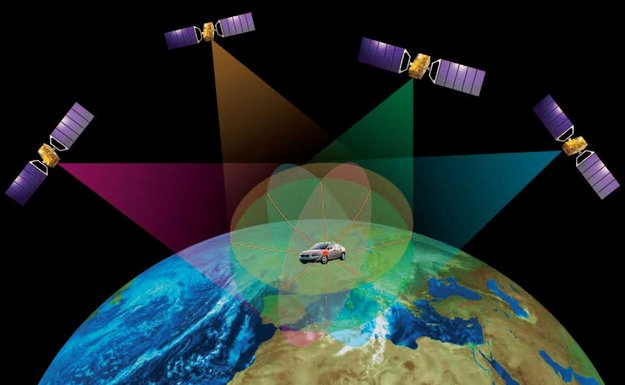
\includegraphics[width=0.6\textwidth]{pictureNav}
		\caption{Satelitska navigacija\cite{bookProcessing} }
		\label{Fig:nn}
		
	\end{figure}
	%http://www.academia.edu/12873735/PRIMJENA_GPS_GLOBALNI_NAVIGACIJSKI_SISTEM_i_GNSS_GLOBALNI_NAVIGACIJSKI_SATELITSKI_SISTEM_U_GEOLO%C5%A0KOM_KARTIRANJU_I_IZRADI_IN%C5%BDENJERSKO-GEOLO%C5%A0KIH_KARATA_NA_PRIMJERU_KLIZI%C5%A0TA_JUNUZOVI%C4%86I_SREBRENIK
	%primjena u kartografiji
	Spominjući GNSS, najčešće se misli na \textit{"sazviježđe"}
	satelita koji odašilju signale, potrebne za određivanje trenutne pozicije, i \textit{Navigacijske poruke} (engl. Navigation Messages (NM)).
	\textit{"Sazviježđe"} satelita predstavlja (1) svemirski segment GNSS sustava.
	Postoji još (2) kontrolni segment koji čine kontrolne stanice smještene na Zemlji i (3) korisnički segment, tj. GNSS prijemnici (Slika \ref{Fig:GNSSsegmenti}).
	Kontrolni segment nadzire i upravljaja radom sustava.
	
	\begin{figure}[h]
			\centering
			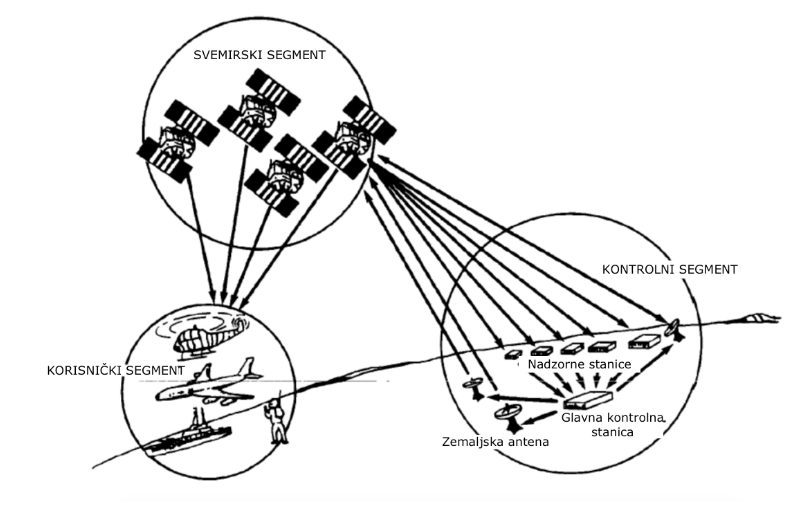
\includegraphics[width=0.6\textwidth]{GNSSsegmenti}
			\caption{Segmenti GNS sustava (GNSS)} %https://dr.nsk.hr/islandora/object/fpz%3A511/datastream/PDF/view
			\label{Fig:GNSSsegmenti}
			
	\end{figure}
	
	Trenutno postoji više GNS sustava (GNSS). Neki su u potpunosti 
	operativni, a neki samo djelomično.
	Najraširaniji u civilnoj upotrebi je GPS (Global Positioning System).
	GPS je u potpunosti operativan i u vlasništnu Vlade SAD-a. Njime upravlja Ministarstvo obrane SAD-a (engl. US Air Force).
	GPS omogućava dvije znatno različite razine korištenja, civilnu i vojnu.
	Vojna razina korištenja pruža mogućnosti, a dopuštena je samo određenim 
	korisnicima. Civilna razina korištenja je dostupna svima, bez dodatne naknade, uz uvjet posjedovanja GPS-prijemnika. 
	
	Drugi, također u potpunost operativan GNSS, je GLONASS (Global'naya Navigatsionnaya Sputnikovaya Sistema) koji je u vlasništvu Rusije.
	Postoje i GNSS sustavi u razvoju. Jedan od njih je Galileo.
	Galileo-om upravlja Europska unija (EU). Najavljeno je da će postati u potpunosti operativan do 2020 \cite{bookProcessing}.
	Kina posjeduje lokalni navigacijski satelitski sustav BeiDou 
	na kojemu se radi da postane globalni najkasnije do 2020\cite{bookProcessing}.
	
	Primjena GNSS-a dijeli se na pozicioniranje i navigaciju.
	\begin{defn}[Navigacija]
		Navigacija obuhvaća trenutno određivanje položaja i brzine entiteta u pokretu.
		Svrha navigacije je praćenje i upravljanje gibanja entiteta.
	\end{defn}
	
	\begin{defn}[Pozicioniranje]
		Pozicioniranje nazivamo postupak određivanja položaja točkovnog entiteta ili niza 
		točkovnih entiteta u prostoru.
	\end{defn}
	Ovaj rad se bavi isključivo bespojenom (engl. off-line) navigacijskom primjenom, u svrhu praćenja entiteta.
	Bespojena navigacija se koristi u prometnoj znanosti u analizi prometnih puteva. Kako ne zahtjeva izračunavanje u realnom vremenu (engl. real-time),
	svodi se na određivanje položaja točkovnog entiteta koji je statičan u danom vremenu $t$, tj. pozicioniranje.
	Određujući položaj entiteta za niz vremena $ t_1,t_2, \hdots ,t_n $, dobiva se 
	aproksimacija kretanja entiteta u vremenskom okviru $[t_1,t_n]$.
	Preciznost aproksimacije kretanja zadaje se veličinom okvira i parametrom $n$, ili dostupnošću podataka.
	Praksa ne zathjeva da je $n$ u odnosu na vremenski okvir duljine 1 sata prevelik.
	Točno kretanje entiteta moguće je
	odrediti preslikavanjem dobivene aproksimacije na kartu prometnih puteva.
	U tu svrhu se koriste otprije poznati algoritmi.
	Dakle, u ovom radu se bavi algoritmom za pozicioniranje (statičkog entiteta)
	u konceptu jednog određenog GNSS-a, GPS-a u aspektu civilne razine korištenja.
	
	%TODO sto koje poglvlje donosi
	
\chapter[Globalni pozicijski sustav (GPS)][GPS]{Globalni pozicijski sustav (GPS, engl. Global Positioning System)}
	Sazvježđe GPS-a se sastoji od najmanje 24 satelita raspoređenih u 6 jednako odmaknutih orbita, svaka s inklanacijom od $55$ stupnjeva od ekvatorijalne
	ravnine (engl. Medium Earth Orbit (MEO)).
	Sateliti kruže na visini od oko 20200 kilometara od Zemljine površine s periodom rotacije 12 zvjezdanih sati. 
	Sateliti su raspoređeni na način da u svakom trenutku za svako mjesto na Zemljinoj površini postoje barem 4 dostupna satelita. Definicija dostupnosti satelita je dana u kasnijem teksu (Stranica \pageref{stranica:dostupnost}).
	
	Svi GPS sateliti odašilju signale na istoj osnovnoj frekvenciji/frekvencijama (Slika \ref{Fig:GPSSignal}). 
	U satelitima, vrijeme je praćeno pomoću cezijevih satova koji se sinkroniziraju s univerzalnom GPS atomskom vremenskom skalom. Sinkronizacija se odvija u periodima.
	\begin{figure}[H]
		\centering
		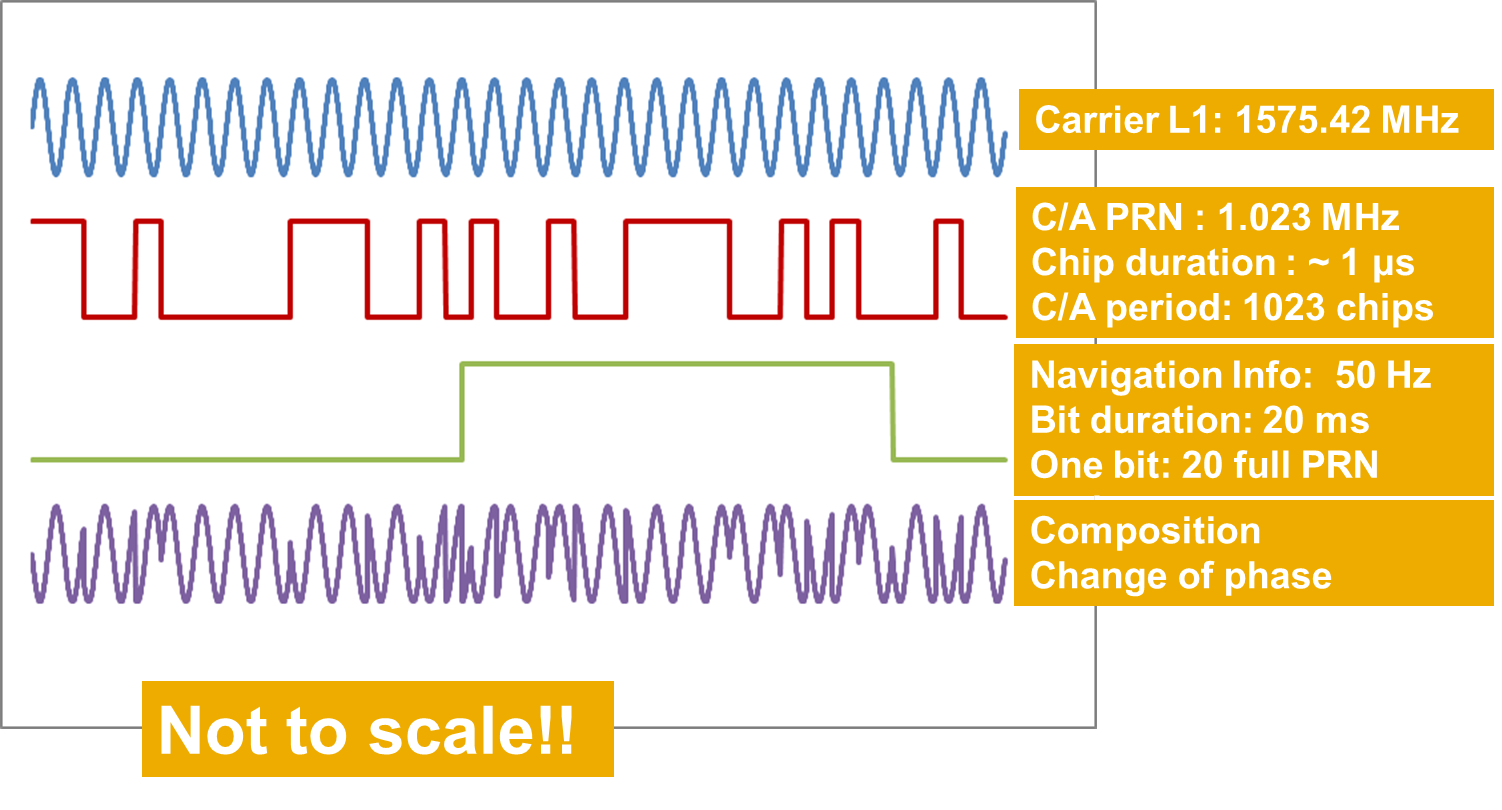
\includegraphics[width=0.4\textwidth]{GPS_Signals}
		\caption{GPS signal i njegove komponente \cite{GPS:1}}
		\label{Fig:GPSSignal}
	\end{figure}
	
	\section[C/A PRN kod]{GPS signali: C/A PRN i P kod}
	\subsection{C/A PRN kod i primjene}\label{CAkod}
	GPS sateliti odašilju signale na dvije frekvencije (nosača) $L_1$ i $L_2$, od kojih je $L_1$ na 1575.42 MHz namjenjena civilnoj upotrebi. Pojam signal se često u satelitskoj navigaciji
	koristi samo za dio GPS signala koja sadržava C/A PRN kod (eng. Coarse Acquisition Pseudo Random Noise). 
	Svaki satelit posjeduje jedinstveni C/A PRN kod koji predstavlja niz 0 i 1 duljine 1023 bit-a.
	GPS-prijemnik razlikuje signale ( signale koji sadrže podatke potrebne za određivanje položaja i \textit{Navigacijske poruke}) različitih satelita
	temeljem sadržanih C/A PRN kodova. Satelit C/A PRN kodove odašilje neprestano, s početkom na početku svake sekunde. Prijemnik primljeni C/A PRN kod korsti za 
	razlikovanje satelita odašiljetelja, ali i za računanje pseudo-udaljenosti.
	
	\begin{defn}[Pseudo-udaljenost]
		Naka su svi sateliti numeriraniprirodnim  brojevima s početkom 
		u 1. Naka je $\mathbf{i} \in \mathbb{N}$ neki satelit i $\mathbf{t}$ prijemnik
		koji je u mogućnosti primiti signal koji odašilje satelit $\mathbf{i}$. Pseudo-udaljenost
		između satelita odašiljatelja $\mathbf{i}$ i prijemnika primatelja $\textbf{t}$:
		$$d_i = c\cdot(t'_i- t_i)$$
		gdje je c konstanta koja je jednaka (prosječnoj) brzini putovanja signala od satelita do prijemnika. $t'_i$ je vrijeme primanja signala, a $t_i$ vrijeme slanja signala
		(po UTC vremenu).
	\end{defn}
	\textbf{Pseudo-udaljenost} je aproksimacija udaljenosti između satelita odašiljatelja i prijemnika primatelja signala u određenom trenutku.
	Neka je $\delta t := (t'_i- t_i)$. Vrijeme putovanja signala izračunava se poravnavanjem odgovarajućih dijelova signala, tj. C/A PRN kodova.
	Naime, prijemnik i satelit istovremeno generiraju isti C/A PRN kod. Budući da 
	dok signala putuje, prijemnik još uvijek generira C/A PRN kod, po primitku signala,
	ta 2 koda se uspoređuju, poravnavaju. Temeljem razlike u poravnanju, dobivenog i generiranog C/A PRN koda,
	računa se procjena vremena putovanja, tj. $\delta t$ (Slika \ref{fig:deltat}).
	\begin{figure}[H]
		\centering
		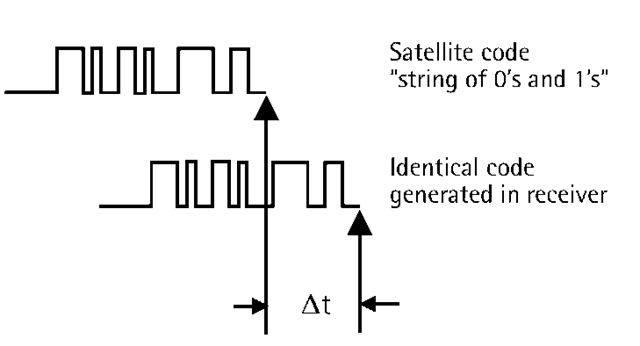
\includegraphics[width=0.4\textwidth]{deltat}
		\caption{Procjena vremena putovanja signala ($\delta t$)}
		\label{fig:deltat}
	\end{figure}
	Za vrijednost konstante $c$ se uzima brzina svjetlosti koja predstavlja brzinu putovanja poruke satelita u vakuumu. Ona dovoljno dobro modelira stvarnu prosječnu brzinu putovanja.
	
	Budući da se psudo-udaljenost dobiva poravnavanjem kodova\label{stranica:kodno},
	upravo opisani način određivanja pseudo-udaljenosti naziva se kodni.
	
	Postoji još i fazni način određivanja psudo-udaljenosti koji se zasniva na poravnanju valova nosača (engl. Carrier phase) nakon micanjem C/A PRN i P(Y) kodova  iz poruke (Slika \ref{Fig:GPSSignal}).
	Fazno mjerenje služi kao nadopuna kodnom mjerenju u svrhu poboljšanja točnosti određivanja položaja.
	
	
	\section{P kod}\label{Pkod}
	P kod je dio GPS signala koji se odašilje na obje frekvencije i rezerviran je za vojnu razinu upotrebe.
	Kao i C/A PRN kod, sastoji se od niza nula i jedinica i šalje se brzinom 1023 bit/s, ali je znatno dulji.
	Potrebno je ukupno 37 tjedana kako bi se sekvencijalno poslao cjelokupni P kod.
	Za razliku od C/A koda, gdje svaki satelit ima svoj jednistveni C/A kod, P kod je
	distribuiran među satelitima. Isječci P koda koji pripadaju različitim satelitima međusobno su različiti.
	Svakih 7 dana u točno određeno vrijeme određeni satelit odašilje svoj dio P koda.
	Na taj način, prijemnik razlikuje jedan satelit od drugoga. Npr. ukoliko
	satelit $\mathnormal{S}$ odašilje 14. tjedan P koda, onda je satelit $\mathnormal{S}$
	zapravo \textit{Space Vehicle 14 (SV 14)}.
	Kako bi se rezerviralo korištenje P koda samo za vojnu razinu upotrebe,
	prijemnik signalom ne prima goli P kod, već njegovu kriptiranu verziju, u oznaci $P(Y)$.
	Također, samo korisnicima s vojnom razinom upotrebe se prosljeđuje informacija kako dekriptirati $P(Y)$ u $P$.
	$P$ kod omogućava točnije određivanje pozicije entiteta.
	
	\section{Pogreške određivanja položaja i vrste}\label{sec:pogreske}
	Pogreške određivanja položaja se grubo dijele na dvije vrste: (1)
	pogreške nastale usljed konstrukcije ulaza algoritma i
	(2) usljed primjenje algoritma za određivanje položaja na mjerenim psudo-udaljeniostima.
	Dakle, postoje dva izvora: ulazni podatci algoritma (tip 1) i algoritam (tip 2).
	Izvori pogreške tipa 1 su najčešće pogreške pri određivanju pseudo-udaljenosti
	ili raspoređenost satelita oko Zemlje (Slike \ref{fig:DOP}, \ref{fig:DOPLow} i \ref{fig:DOPHigh}).
	Nepovoljan položaj promatranih satelita može rezultirati skoro pa zavisnim jednadžbama
	u \ref{eq:1}.
	\begin{figure}[H]
		\centering
		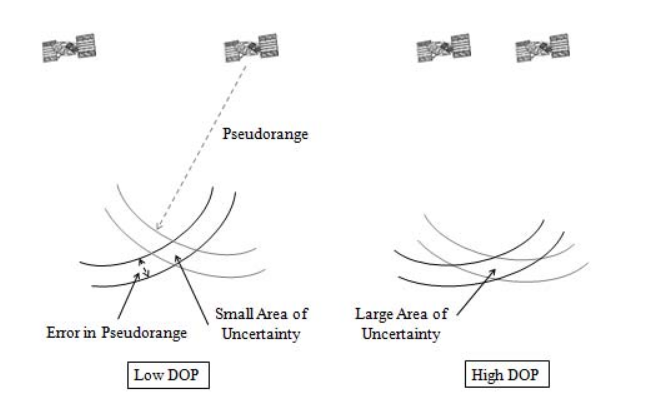
\includegraphics[width=0.6\textwidth]{DOP}
		\caption{Razlike u razmještaju satelita}
		\label{fig:DOP}
	\end{figure}%
	\begin{figure}[H]
		\centering
		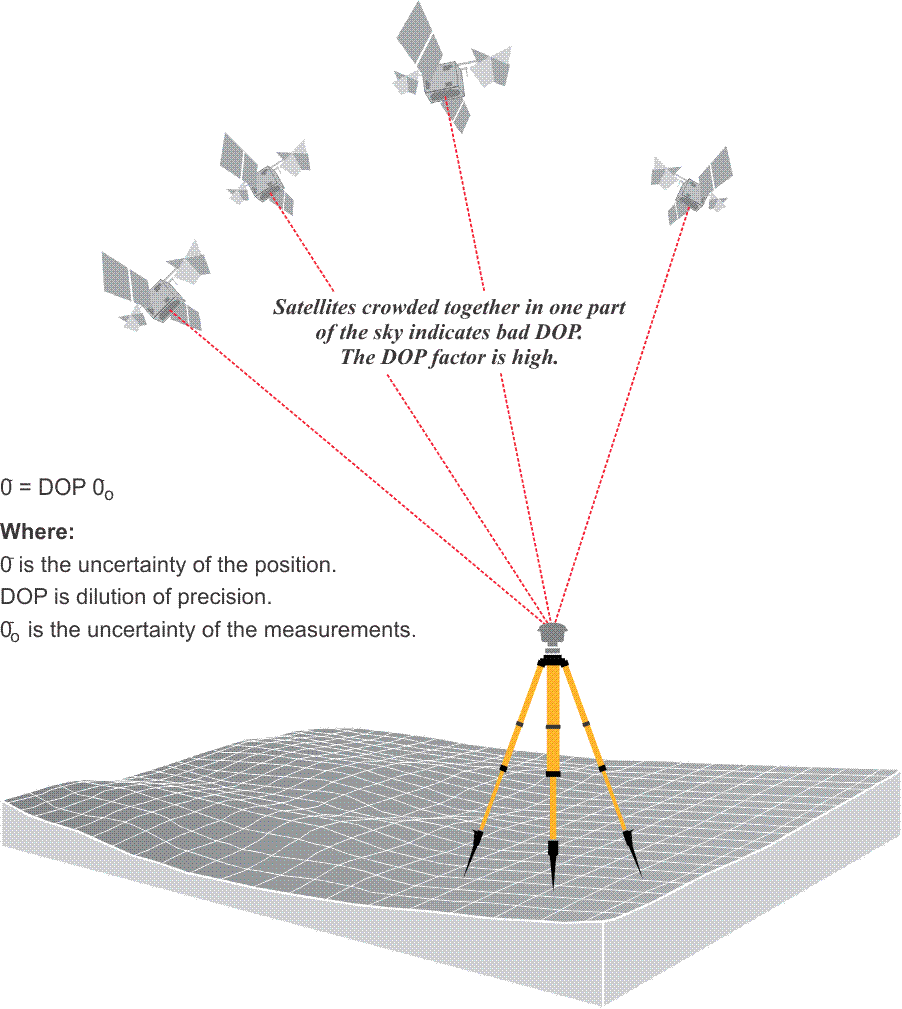
\includegraphics[width=0.6\textwidth]{DOPLow}
		\caption{Loš razmještaj satelita}
		\label{fig:DOPLow}
	\end{figure}%
	\begin{figure}[H]
		\centering
		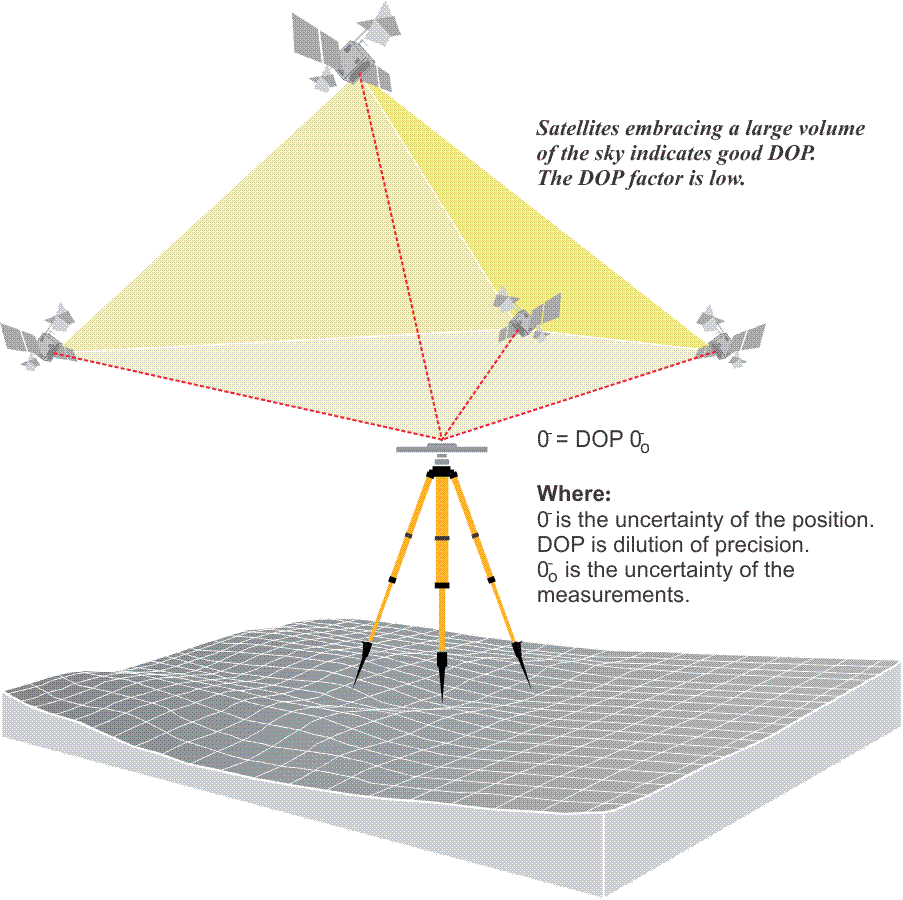
\includegraphics[width=0.4\textwidth]{DOPHigh}
		\caption{Dobar razmještaj satelita}
		\label{fig:DOPHigh}
	\end{figure}
	
	
	
	Detaljnija podjela pogrešaka tipa 1 nastalih 
	pri određivanju psudo-udaljenosti i na što koja utječe dana je sljedećom tablicom.
	
	\begin{table}[h]\centering
		\caption{Pogreške određivanja pseudo-udaljenosti}
		\begin{tabular}{ |p{3cm}|p{4cm}| }
			\hline
			\rowcolor{lightgray} izvor & utjecaj\\[0.5ex]
			\hline\hline
			\multirow{2}{4em}{satelit} & pogreške orbite  \\ 
			& pogreška sata satelita  \\ 
			\hline
			\multirow{2}{4em}{rasprostiranje signala} & troposferska refrakcija  \\ 
			& ionosferska refrakcija  \\
			\hline
			\multirow{2}{4em}{prijemnik} & pogreške antene \\ 
			& pogreška sata  \\ 
			\hline
		\end{tabular}
	\end{table}
	Utjecaj sistemskih pogrešaka otklanja se modeliranjem ili
	kombinacijom opažanja.
	Korištenjem više prijemnika, otkanjaju se pogreške spacifične za satelite.
	Pogreške specifične za prijemnike otkanja korištenje viška satelita.
	Utjecajem troposfere se najčešće otklanja modeliranjem,
	a ionosfere korištenjem dva signala različitih frekvencija.
	
	Uz sistemske pogreške, postoje još i slučajne pogreške nastale zbog trenutnog mjerenja i slučajnog dijela
	višestruke refleksije signala (multipath) nastalog interferencijom 
	direktnog i reflektiranog signala (Slika \ref{fig:multipath}).
	\begin{figure}[H]
		\centering
		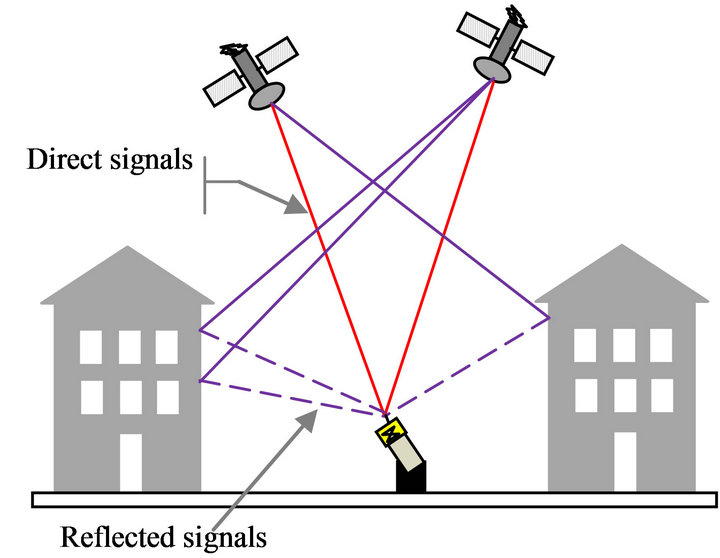
\includegraphics[width=0.4\textwidth]{multipath}
		\caption{Višestruka refleksija signala}
		\label{fig:multipath}
	\end{figure}
	
	Sistemske i slučajne pogreške mogu biti otklonjene koristeći RTK-LIB.
	%RTK LIB u POGLAVLJE 4).
	 Prije konstrukcije ulaza algoritma za određivanja položaja, smatramo da je
	pogreška s izvorom u pseudo-udaljenostima maksimalno reducirana.
	Dakle, pretpostavljamo kako ona više nije značajna
	neuzimajući ju u obzir u daljnjem postupku izračuna položaja. \label{stranica:greskaOvisisamoOxOpravdano}
	Smatramo da koristimo potpuno ispravljene pseudo-udaljenosti.
	
	\vspace{0.5cm}
	Pogreške tipa 2 mogu imati izvor u dizajnu izvedbe algoritma ili samoj izvedbi, npr.
	numeričke greške, greške zbog ograničene preciznosti računala,
	aproksimacije pojedinih vrijednosti.
	
	One se ne modeliraju algoritmima procjene položaja (Poglavlje \ref{sec:algoritam}), već prilikom dizajna izvedbe odabranog algoritma (Poglavlje \ref{sec:izvedba})
	
	U poglavlju \ref{sec:izvedba}, biti će obrađena analiza pogreške tipa 2 za odabrani algoritam.
	
	\section{Navigation Message}\label{sec:NM} %http://what-when-how.com/gps/gps-details/
	Svaki satelit, uz C/A PRN i P kod, odašilje i dodatne podatke potrebne za ispravo pozicioniranje prijemnika. Odašilje ih u obliku \textit{Navigacijske poruke} koja se šalje zajedno s generiranim C/A PRN kodovima (Slika \ref{Fig:GPSSignal}).
	
	Navigacijska poruka se sastoji od 25 okvira \cite{bookProcessing}.
	Jedan okvir se satoji od 5 podokvira i svaki sadržava vrijeme slanja
	sljedećeg okvira (Slika \cite{GPS:1}). Za slanje cjelokupnog podokvira potrebno je 6 sekundi,
	6 cjelokupnih C/A PRN kodova. Prijemnik je u mogućnosti računati pseudo-udeljenost za novu poziciju satelita svakih
	6 sekundi.
	Za slanje cjelokupne NM, potrebno je 12.5 minuta.
	U nastavku termin poruka koristi se misleći na podprozor.
	\vspace{0.5cm}
	
	Prozor sadrži:
	\begin{enumerate}
		\item GPS vremena odašiljanja,
		\item signal prijenosa s P na C/A kod (potpoglavlja \ref{Pkod} i \ref{CAkod}),
		\item podatke o orbitalnoj putanji satelita,
		\item podatke o korekciji sata satelita,
		\item almanah statusa svih satelita u sazvježđu,
		\item koeficijente preračunavanja GPS vremena u UTC,
		\item ionosferski model korekcije za koji se smatra da je potrebno koristiti.
	\end{enumerate}
	
	\begin{defn}[Universal Time Coordinate (UTC vrijeme)]
		Universal Time Coordinate je vremenski standard zasnovan na međunarodnom atomskom vremenu koji se najčešće koristi u znanstvene i vojne svrhe. Drugi nazivi za taj vremenski standard su ZULU vrijeme i Greenwich Mean Time (GMT).
	\end{defn}
	
	\begin{figure}[H]
		\centering
		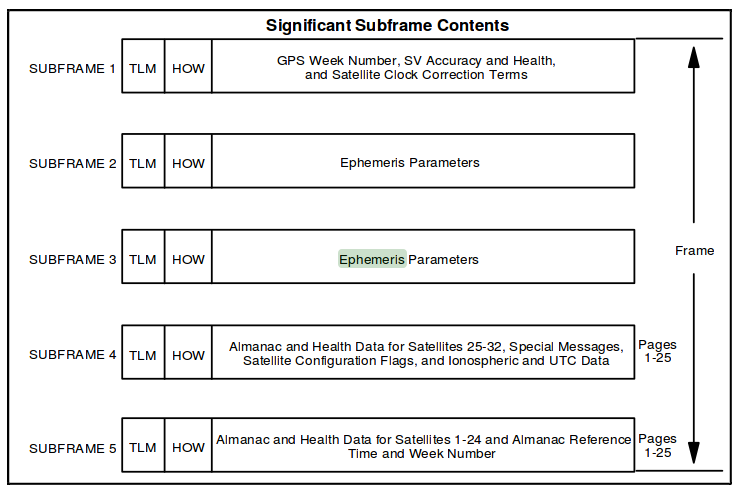
\includegraphics[width=0.6\textwidth]{NACONTENT}
		\caption{Pregled strukture prozora navigacijske poruke\cite{GPS:1}}
		\label{Fig:aaa}
	\end{figure}
	Pojedini dijelovi navigacijske poruke pomažu pri otklanjaju pogrešaka tipa 1  
	(Potpoglavlje \ref{sec:pogreske}), određivanju
	pseudo-udaljenosti i trenutnoj poziciji satelita.
	Naime, iz podataka o orbitalnoj putanji satelita moguće je za odabrani trenutak izračunati poziciju (koordinate) satelita u orbitalnom koordinatnom sustavu pa i svakom drugom.
	 
	Za razumjevanje ovoga rada, dovoljno je razumjeti sljedeće.
	Prijemnik svakih 6 sekundi ima dovoljno podataka da odredi novu pseudo-udaljenost do istog satelita sve dok on ne prestane biti dostupan. 
	
	\begin{defn}[Dostupnost satelita $\mathnormal{S}$ prijemniku $\mathnormal{T}$]
		\label{stranica:dostupnost}
		Za satelit $\mathnormal{S}$ kažemo da je dostupan prijemniku $\mathnormal{T}$ u trenutku $\mathnormal{t}$ ako je u sljedećih 6 sekundi u mogućnosti izračunati
		pseudo-udaljenost do satelita $\mathnormal{S}$ i konstruirati sljedeću jednadžbu:
		\begin{align}\label{eq:position1}
		d_s = \sqrt{(x-x_s)^{2}+(y-y_s)^{2}+(z-z_s)^{2}}
		\end{align}
		gdje su jedine nepoznanice $(x,y,z)$, tj. koordinate položaja prijemnika.
		$(x_s,y_s,z_s)$ su koordinate položaja satelita. 
	\end{defn}
	
	\section{Proces određivanja položaja}\label{sec:positionProcess}
	U pravilu, u svakom trenutku, prijemnik ima više dostupnih satelita od kojih dobiva poruke. Za određivanje položaja prijemnika u granicama dopuštene točnosti, %TABLICA
	zahtjevaju se barem 4 dostupna satelita\label{stranica:4satelita}.
	
	Kako bi prijemnik odredio svoju poziciju računa tri nepoznanice: geografsku širinu, duljinu i nadmorsku visinu.
	Neka je $k$ broj vidljivih satelita od prijemnika $\mathnormal{T}$.
	Prijemnik $\mathnormal{T}$ promatrajući poruke dobivene od samo jednog satelita,
	u vremenu $\mathnormal{t}$, izračunava samo jednu pseudo-udaljenost i može konstruirati samo jednu jednadžbu \ref{eq:position1}
	 koja mu omogućava odrediti sferu oko promatranog satelita na kojoj bi se mogao nalaziti (Slika \ref{Fig:1SatelitePosition}).
	
	\begin{figure}[H]
		\centering
		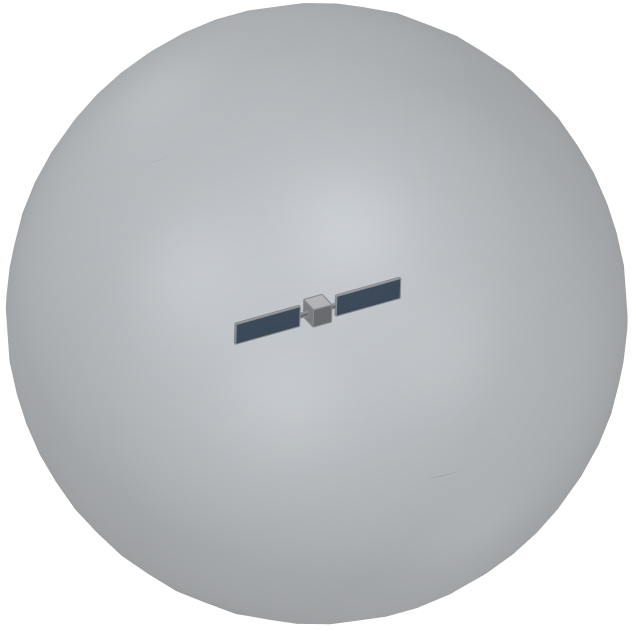
\includegraphics[width=0.4\textwidth]{satellite_distance_13D}
		\caption{Sfera oko promatranog satelita na kojoj bi se prijemnik mogao nalaziti \cite{gps:2}}
		\label{Fig:1SatelitePosition}
	\end{figure}
	Uključujući u izračun pridobivene pseudo-udaljenosti od još jednog satelita dobivamo situaciju prikazanu na Slici \ref{Fig:2SatelitePosition}.
	\begin{figure}[H]
		\centering
		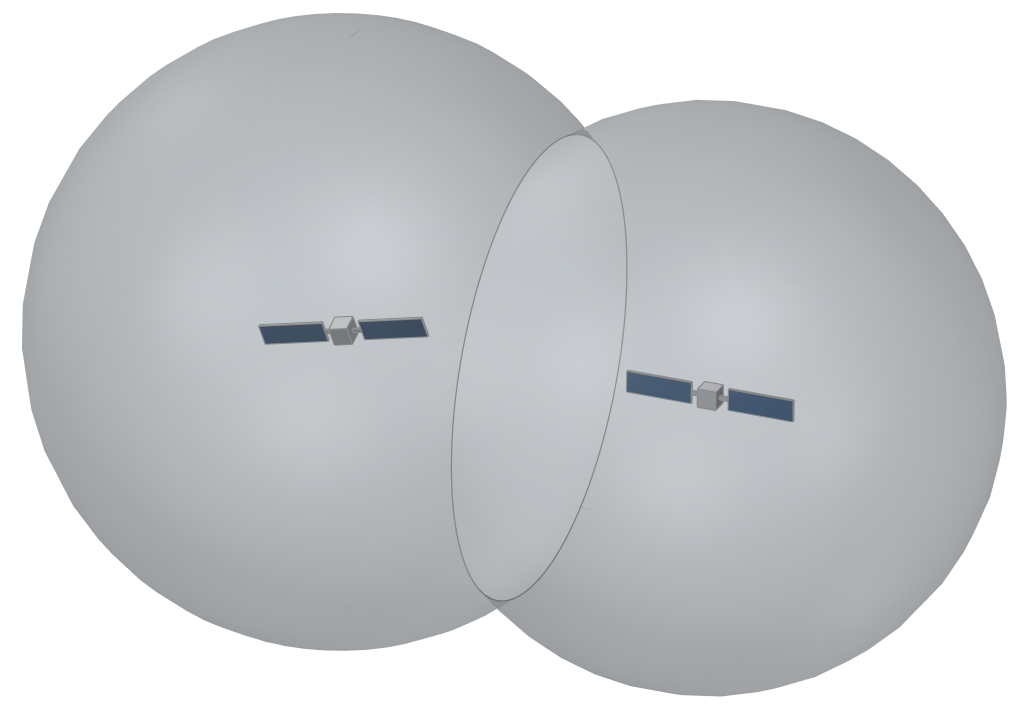
\includegraphics[width=0.6\textwidth]{satellites_distance_23D}
		\caption{Sfere oko 2 promatrana satelita, presjek je kružnica na kojoj bi se prijemnik mogao nalaziti. \cite{gps:2}}
		\label{Fig:2SatelitePosition}
	\end{figure}
	Uključujuči u izračun još jedan satelit, dobivamo situaciju prikazanu na Slici \ref{Fig:3SatelitePosition}.
	
	\begin{figure}[H]
		\centering
		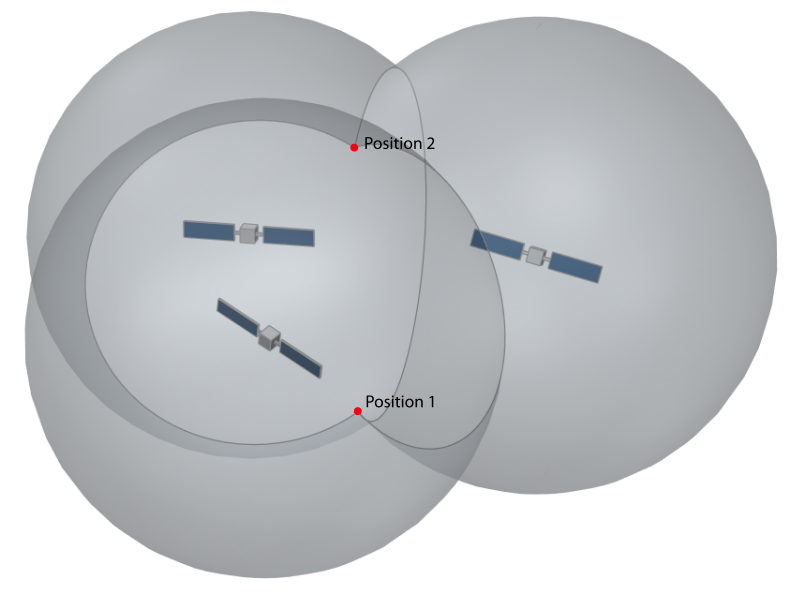
\includegraphics[width=0.6\textwidth]{satellites_distance_33D}
		\caption{Sfere oko 3 promatrana satelita, presjek su 2 točke na kojoj bi se prijemnik mogao nalaziti. \cite{gps:2}}
		\label{Fig:3SatelitePosition}
	\end{figure}
	
	Presjek 3 promatrane sfere su 2 točke na kojoj bi se prijemnik mogao nalaziti.
	Jedna točka se nalazi daleko u svemiru, dok je druga točka točka kandidat pozicije prijemnika. 
	
	Algebarski, rješavamo sljedeći sustav linearnih jednadžbi u $(x,y,z)$ :
	\begin{align}\label{eq:position2}
	 d_1 = \sqrt{(x-x_1)^{2}+(y-y_1)^{2}+(z-z_1)^{2}} \notag \\
	 d_2 = \sqrt{(x-x_2)^{2}+(y-y_2)^{2}+(z-z_2)^{2}} \\
	 d_3 = \sqrt{(x-x_3)^{2}+(y-y_3)^{2}+(z-z_3)^{2}} \notag
	\end{align}
	gdje su $1,2 \text{ i }3$,  3 različita satelita, a $(x_i,y_i,z_i)$ pripadajuće
	koordinate položaja satelita u (ECEF XYZ) koordinatnom sustavu.
	ECEF XYZ koordinatni sustav je prikazan na Slici \ref{Fig:na}. Ishodište (ECEF XYZ) koordinatnog sustava je središte zemlje.
	
	\begin{figure}[H]
		\centering
		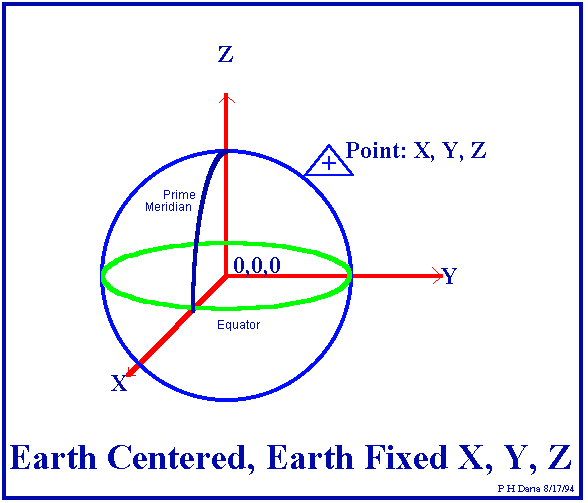
\includegraphics[width=0.6\textwidth]{ecefxyz.png}
		\caption{Earth-Centered, Earth-Fixed $\mathnormal{X}$, $\mathnormal{Y}$, $\mathnormal{Z}$ coordinate system ( ECEF XYZ koordinatni sustav ) \cite{GPS:overview}}
		\label{Fig:na}
	\end{figure}
	
	Svaki prijemnik je sposoban izvesti konverziju iz i u koordinata u ECEF XYZ sustavu 
	u i iz geografskih (geografska širina, duljina i nadmorska visina) \cite{GPS:overview}.
	Dakle, prijemniku su potrebna barem 3 dostupna satelita kako bi odredio poziciju.
	Ali se ipak na stranici \pageref{stranica:4satelita} se postavlja zahtjev na barem 4. 
	
	Primjetimo kako proces određivanja položaja prijemnika
	indirektno zahtjeva usklađenost satova prijemnika i dostupnih satelita.
	Satovi svih satelita su međusobno usklađeni usklađenošću s GPS vremenom. Ukoliko odstupanje ipak postoji, biti će zapisano u navigacijskoj poruci pa se može uzeti u obzir prilikom određivanja položaja prijemnika.
	Napomenimo, GPS vrijeme nije jednako UTC vremenu. GPS vrijeme je bilo 0 u 06.01.1980. i određeno je protjecanjem vremena u GPS satelitima, tj. njihovim 
	satovima. 
	
	Satovi prijemnika nisu iste preciznosti kao satovi satelita.
	Prijemnici obično koriste satove preciznosti do otprilike $10^{-6}$ sekundi.
	Pogreška određivanja vremena od $10^{-6}$ sekundi dovodi do pogreške u
	određivanju pseudo-udaljenosti od oko 300 metara.
	Uključijući u izračin i pogrešku sata prijemnika, pseudo-udaljenost modeliramo jednadžbom:
	$$d_i = c\times(t'_i- t_i+ d_T)$$
	gdje $d_T$ predstavlja spomenutu pogrešku.
	Budući da se prilikom određivanja položaja, 
	spomenuta pogreška u oznaci $d_T$ ne mijenja u odnosu na satelit koji se promatra,
	može se izračunati dodavajući ju kao nepoznanicu u sustav jednadžbi \ref{eq:position2}
	Dakle, sustav jednadžbi \ref{eq:position2} prelazi u:
	\begin{align}\label{eq:position3}
	d_1 = \sqrt{(x-x_1)^{2}+(y-y_1)^{2}+(z-z_1)^{2}} + c\cdot d_T \notag \\
	d_2 = \sqrt{(x-x_2)^{2}+(y-y_2)^{2}+(z-z_2)^{2}} + c\cdot d_T  \\
	d_3 = \sqrt{(x-x_3)^{2}+(y-y_3)^{2}+(z-z_3)^{2}} + c\cdot d_T \notag 
	\end{align}
	
	Kako bi za gornji sustav postojala mogućnost pronalaska rješenja,
	uvodi se zahtjev na još barem jedan dostupni satelit, što je ukupno 4 (Stranica \pageref{stranica:4satelita}).
	Dobivamo sljedeći sustav jednadžbi u $(x,y,z,d_T)$:
	\begin{align}\label{eq:1}
	 d_1 = \sqrt{(x-x_1)^{2}+(y-y_1)^{2}+(z-z_1)^{2}} + c\cdot d_T \notag \\
	 d_2 = \sqrt{(x-x_2)^{2}+(y-y_2)^{2}+(z-z_2)^{2}} + c\cdot d_T  \\
	 d_3 = \sqrt{(x-x_3)^{2}+(y-y_3)^{2}+(z-z_3)^{2}} + c\cdot d_T \notag \\
	 d_4 = \sqrt{(x-x_4)^{2}+(y-y_4)^{2}+(z-z_4)^{2}} + c\cdot d_T \notag
	\end{align}
	
	Upravo opisanom postupkom otklanjamo pogrešku nastalu prilikom 
	određivanja pseudo-udaljenosti 
	s izvorom u pogrešci sata prijemnika.
	U praksi se može koristiti još veći broj dostupnih satelita što poboljšava 
	preciznost pozicioniranja prijemnika. Očekivana pogreška rješenja dobivenog rješavanjem sustava\ref{eq:1} je između $10^2$ i $10^3$. Tako dobiveno rješenje se profinjuje čime se postiže pogreška veličine $10^1$.
	Ovim radom se proučava, opisuje, dizajnira i izvodi algoritam za rješavanje sustava \ref{eq:1}.
	Naime, rješavanje sustava \ref{eq:1} čini temelj procesa određivanja položaja, nužno ga je provesti.
	Za primjene koje zahtjevaju malu točnost, ono je i dovoljno.\\
	Metode za profinjavanje dobivenog rješenja mogu biti izrazito kompleksne i ovise o primjeni. Svojom kompleksnošću i raznovrsnošću prelaze obim ovoga rada.\\

\chapter[Algoritam procjene položaja (APP)]{Algoritam procjene položaja u domeni navigacijske primjene}\label{sec:algoritam}

\textit{Algoritam procjene položaja u domeni navigacijske primjene} (APP)
smatramo svakim algoritmom koji za sustav jednadžbi \ref{eq:1}
određuje nepoznatu poziciju prijemnika u koordinatama $(x,y,z)$.
Broj jednadži sustava može biti i veći od 4. Tada govorimo o prezasićenim sustavima.
Ovisno o odabiru, APP se može temeljiti na rješavanju sustava nelinearnih jednadžbi pronalaženjem rješenja pomoću (1) metode najmanjih kvadrata (Newton-ova metoda),
(2) metode zatvorene forme, (3) metode najbližeg susjeda \cite{math:positioning}. 

Općenito, rješava se moduficiran sustav jednadžbi \ref{eq:1} uz $d = c \cdot d_T$:\\
\begin{align}\label{eq:new}
d_1 = \sqrt{(x-x_1)^{2}+(y-y_1)^{2}+(z-z_1)^{2}} +d + v_1\notag \\
d_2 = \sqrt{(x-x_2)^{2}+(y-y_2)^{2}+(z-z_2)^{2}} +d + v_2 \\
d_3 = \sqrt{(x-x_3)^{2}+(y-y_3)^{2}+(z-z_3)^{2}} +d + v_3\notag \\
d_4 = \sqrt{(x-x_4)^{2}+(y-y_4)^{2}+(z-z_4)^{2}} +d + v_4\notag
\end{align}
u koji uključejemo nepoznati parametar $(v_1,v_2,v_3,v_4)$, dodatnu pogreška
izračuna.

Uz oznake 
\begin{align}
\mathbf{\rho} := (d_1, d_2, d_3, d_4)^T \\ 
\mathbf{x} := (x,y,z,d_T)^T \\ 
\mathbf{s}_i := (x_i,y_i,z_i)^T \\ 
\mathbf{h} (\mathbf{x}) := 
\begin{bmatrix}
||(s_1-\mathbf{x}_{1:3})|| + x_4\cdot c\\
||(s_2-\mathbf{x}_{1:3})|| + x_4\cdot c\\
||(s_3-\mathbf{x}_{1:3})|| + x_4\cdot c\\
||(s_4-\mathbf{x}_{1:3})|| + x_4\cdot c
\end{bmatrix} \\
\mathbf{v} := (v_i,v_2,v_3,v_4)^T \label{eq:v}
\end{align}%
prelazi u
\begin{align}\label{eq:matrix}
\mathbf{\rho} = \mathbf{h}(\mathbf{x})+\mathbf{v}
\end{align}%
\section{Iterativna metoda najmanjih kvadrata}

Primjetimo kako je $\mathbf{h}(\mathbf{x})$ jednako pravom vektoru pseudo-udaljenosti (udaljenosti, ako pogreška sata, $d_T$ = 0) između
satelita i prijemnika za prave vrijednosti $\mathbf{x}$,$\bar{\mathbf{x}}$.\\
%Na ovoj razini, 
Algoritam oderđivanja položaja se ne bavi pogreškama tipa 2,
već samo pogreškama tipa 1 (Stranica \ref{stranica:greskaOvisisamoOxOpravdano}).
Također, može se pretpostavti kako su otklonjene sve pogreške tipa 1 koje imaju izvor 
u pogreškama izračuna pseudo-udaljenosti (osim pogreški sata prijemnika) (Stranica \ref{stranica:greskaOvisisamoOxOpravdano}).
Ostaje samo modelirati pogreške koje imaju za izvor trenutni položaj satelita dostupnih za
izračunavanje željenog položaja $\bar{\mathbf{x}}_{(1:3)}$.
U tu svrhu modeliramo vektor pogrešaka $\mathbf{v}$, funkcijom $\mathbf{p}(\mathbf{x})$ koja ovisi o nepoznatom parametru $\mathbf{x}$.
Uz oznaku $\mathbf{y} := \rho$, 
 jednadžba  \ref{eq:matrix} prelazi u
\begin{align}\label{eq:matrix2}
\mathbf{y} = \mathbf{\rho} = \mathbf{h}(\mathbf{x})+ \mathbf{p}(\mathbf{x})
\end{align}%
Preciznije,
član $\mathbf{p}(\mathbf{x})$ modelira pogrešku razlike u procjeni parametra $\mathbf{x}$ od stvarne vrijednosti.
Što je aproksimacija potrebnih vrijednosti za izračun rješenja matrične jednadžbe
\ref{eq:matrix} točnija, to je $\mathbf{p}(\mathbf{x})$ 
bliže nuli za pravu vrijednost $\bar{\mathbf{x}}$.
Aproksimaciju za $\bar{\mathbf{x}}$, u oznaci $\hat{\mathbf{x}}$, pronalazimo tražeći nultočke funkcije $\mathbf{p}(\mathbf{x})$.
U praksi je uobičajeno da mjerenja sadrže pogreške i tada $\mathbf{p}(\mathbf{x})$ uopće ne mora imati 
nultočke i $\hat{\mathbf{x}}$ ne možemo pronaći tražeći nultočke funkcije $\mathbf{p}(\mathbf{x})$.

Ideja metode najmanjih kvadrata je pronalazak $\hat{\mathbf{x}}$ tražeći minimum $\mathbf{p}(\mathbf{x})$, tj.
\begin{align}\label{eq:minimization}
	\hat{\mathbf{x}} = \text{arg min}_\mathbf{x} \mathbf{p}(\mathbf{x})^T\mathbf{p}(\mathbf{x})
\end{align}
Problem opisan jednadžbom \ref{eq:minimization} nije linearan pa
ne postoji općeniti način pronalaska njegovog rješenja.

U slučaju kada su funkcija koju treba minimiziati i početna vrijednost $\mathbf{x}_0$
(iterativnog postupka) dovoljno dobre (vidi: dodatak \ref{appendix:aTay}), rješenja problema \ref{eq:minimization} možemo
dobiti iterativnim postupakom.
Ideja iterativnog postupka je počevši s $\mathbf{x}_0$ računati $\mathbf{x}_1, \mathbf{x}_2, \hdots $ sve dok se novoizračunate vrijednosti ne prestanu mijenjati ili postanu dovoljno bliske prethodnoj, tj.
$\left \| x_{k} - \mathbf{x}_{k-1}\right\| < \delta$ za dovoljno male $\delta > 0$.
$\delta$ još nazivamo i zaustavni kriterij.

Jedan iterativni postupak rješavanja problema \ref{eq:minimization} je Newton-Gaussova metoda (iterativna metoda najmanjih kvadrata).
Newton-Gaussova metoda linearizira $\mathbf{p}(\mathbf{x})$ u okolini od $\mathbf{x_k}$ pomoću prvog člana razvoja funkcije u Taylorov red\label{stranica:NGLin} u točki $\mathbf{x}_k$:
\begin{align}\label{eq:approx}
	\mathbf{p}(\mathbf{x_k}+ \Delta \mathbf{x_k}) \approx \mathbf{p}(\mathbf{x_k}) + \mathbf{p}'(\mathbf{ x_k})\cdot \Delta \mathbf{x_k}
\end{align}

$\Delta \mathbf{x_k}$ se odabire na način tako da
$$lim_{k \to \infty} \left( \mathbf{p}(\mathbf{x_k}) \right) = 0$$ 
jer za pravu vrijednost $\mathbf{x}$ izraz $\mathbf{p}(\mathbf{x}) = 0$ ili poprima svoj minimum ukoliko postoje pogreške
točnosti vrijednosti koje se koriste prilikom konstrukcije sustava.
 
Sada, za $\mathbf{p}(\mathbf{x_{k+1}}) := \mathbf{p}(\mathbf{x_k}+ \Delta \mathbf{x_k}) \approx \mathbf{p}(\mathbf{x_k}) + \mathbf{p}'(\mathbf{x_k})\cdot \Delta \mathbf{x_k}$ želimo
 da je što bliže 0.
 Dakle, $ \Delta \mathbf{x_k} $ odabiremo trežeći minimum funkcije
\begin{align}\label{eq:minDelta}
	\mathbf{p}(\mathbf{x_k}) + \mathbf{p}'(\mathbf{x_k})\cdot \Delta \mathbf{x_k}
\end{align}
u $\Delta \mathbf{x_k}$.

Označimo sada s $J_k := \mathbf{p}'(\mathbf{x_k}) = \mathbf{h}'(\mathbf{x_k})$.
\ref{eq:minDelta} prelazi u 
\begin{align}\label{eq:minDelta2}
	J_k \Delta \mathbf{x_k} +\mathbf{p}(\mathbf{x_k})
\end{align}
čij je minimun dan s (vidi stranicu \pageref{stranica:nastavakLS})  
\begin{align}\label{eq:minDeltaRj}
\Delta \mathbf{x_k} = - (J_k^TJ_k)^{-1}J_k^T \mathbf{p}(\mathbf{x_k})
\end{align}
Izraz za $\mathbf{x_{k+1}}$ je sljedeći:
\begin{align}\label{eq:iter}
	\mathbf{x_{k+1}} = \mathbf{x_{k}} - (J_k^TJ_k)^{-1}J_k^T \mathbf{p}(\mathbf{x_k})
\end{align}
Prilikom izvedbe algoritma, potrebano je pametno odrediti početnu vijednost $\mathbf{x_0}$, te kasnije iterirati po formuli \ref{eq:iter}.
Ukoliko odaberemo dovoljno dobar $\mathbf{x}_0$, dovoljno blizu rješenju i
ako je druga derivacija od $p$ u točki $\bar{\mathbf{x}}$ dovoljno mala,
niz $x_0,x_2, \hdots$ konvergira prema $\bar{\mathbf{x}}$. Izračun $J_k$ za idealan slučaj $d = 0$ se može naći u prilogu \ref{appendix:aTay}.

Algoritam iterativne metode najmanjih je dan u nastavku.

\begin{algorithm}[H]
	\KwData{ $\mathbf{p(\mathbf{x})}, \mathbf{x}_0, \delta$ }
	\KwResult{ $\hat{\mathbf{x}} $ }
	$k = 0$ \;
	\While{$ \left \| \mathbf{x}_{k} - \mathbf{x}_{k-1}\right\| \geq \delta $}{
		$J_k = \mathbf{p}'(\mathbf{x}_k)$ \;
		$\Delta \mathbf{x}_k = - J_k^{-1} \cdot \mathbf{p}(\mathbf{x}_k) $ \;
		$\mathbf{x}_{k+1} =\mathbf{x}_k + \Delta \mathbf{x}_k$ \;
	$k ++$\;
	} 
	$\hat{\mathbf{x}} = \mathbf{x_k}$
\caption{Iterativna metoda najmanjih kvadrata}
\label{code:iterLSM}
\end{algorithm}

Prilikom korištenja gornjeg algoritma za određivanje pozicije entiteta, za $\mathbf{x}_0$ se mogu uzeti koordinate središta zemlje jer su jednadžbe za određivanje položaja dovoljno bliske linearnima.

Ako je poznato da su vrijednosti koje koristimo za konstrukciju
jednadžbi za određivanje položaja \ref{eq:1} za pojedine jednadžbe točnije,
pametno je dati prednost tim jednadžbama pred ostalima.
Važnost pojedine jednadžbe simuliramo pridavanjem težina pojedinoj jednadžbi.
Jednadžbi se pridružuje težina $\sigma_i$ koja je proporcionalna preciznosti 
vrijednosti korištenih prilikom njezine konstrukcije.
Najčešće način pronalaženja odgovarajućih težina je
korištenjem kovarijancone matrice
vektora pogrešaka $\mathbf{v}$ (Jednadžba \ref{eq:v}),u oznaci $\Sigma : = cov(\mathbf{v})$. Minimizacijski problem \ref{eq:minimization} prelazi u %
\begin{align}\label{eq:minimisation2}
\hat{\mathbf{x}} = \text{arg min}_\mathbf{x} \mathbf{p}(\mathbf{x})^T \Sigma^{-1} \mathbf{p}(\mathbf{x})
\end{align}%
Sada, algoritam \ref{code:iterLSM} prelazi u algoritam \ref{code:iterLSMW}.

\begin{algorithm}[H]
	\KwData{ $\mathbf{p(\mathbf{x})}, \mathbf{x}_0, \delta$, $\Sigma$ }
	\KwResult{ $\hat{\mathbf{x}} $ }
	$k = 0$ \;
	\While{$ \left \| \mathbf{x}_{k} - \mathbf{x}_{k-1}\right\| \geq \delta $}{
		$J_k = \mathbf{p}'(\mathbf{x}_k)$ \;
		$\Delta \mathbf{x}_k = - (\Sigma^{-\frac{1}{2}}J_k ) ^{-1} ( \Sigma^{-\frac{1}{2}}(\mathbf{p}(\mathbf{x}_k))$ \;
		$\mathbf{x}_{k+1} =\mathbf{x}_k + \Delta \mathbf{x}_k$ \;
		$k ++$\;
	} 
	$\hat{\mathbf{x}} = \mathbf{x_k}$
	\caption{Iterativna metoda težinskih najmanjih kvadrata}
	\label{code:iterLSMW}
\end{algorithm}
Procjenitelj za $\bar{\mathbf{x}}$ dobiven težinskom metodom najmanjih kvadrata, jednakost \ref{eq:minimisation2}, ima najmanju varijancu među svim procjeniteljima za
$\bar{\mathbf{x}}$. Ukoliko je vektor pogrešaka $\mathbf{v}$ normalno
distribuiran, procjenitelj \ref{eq:minimisation2} postaje procjenitelj
metode najbližeg susjeda (Podpoglavlje \ref{sec:MLE} i MLE procjenitelj).

Prilikom korištenja iterativne metode najmanjih kvadrata potrebno je
modelirati distribuciju vektora pogrešaka, točnije kovarijanconu matricu $\Sigma$.
Također, potrebno je pripazati na 
velike pogreške u određivanju vrijednosti pomoći kojih se gradi sustav jednadžbi 
\ref{eq:1} i netipične vrijednosti ("outlinere") koji se uklanjaju prije primjene algoritma.

Sljedeće poglavlje opisuje izvedbu upravo opisanog algoritma \ref{code:iterLSMW} i 
analizu njegove točnosti. Prije same izvedbe, navodi se zanimljiva posljedica
analize pogreške metode najmanjih kvadrata i pregled još nekih metoda za rješavanje
sustava \ref{eq:1}.
\subsection{Analize pogreške metode najmanjih kvadrata}
Uz oznake kao do sada, neka $\bar{\mathbf{y}}$ predstavlja prave udaljenosti između satelita i promatranog entiteta (prijemnika) i $\hat{\mathbf{y}}$ izračunate pseudo-udaljenosti. 
Vrijedi
$\hat{\mathbf{y}} = \bar{\mathbf{y}} + \Delta \mathbf{y}$.
Promatramo idealan slučaj za metodu iterativnih najmanjih kvadrata (Algoritam \ref{code:iterLSM}), $\delta = 0$.
Neka je $\hat{\mathbf{x}} = \bar{\mathbf{x}} + \Delta \mathbf{x}$ rješenje metode najmanjih kvadarata konvergirala, tj. 
$\hat{\mathbf{x}} = \mathbf{x}_{k'}$ i $\forall m \geq k', \mathbf{x}_m = \mathbf{x}_{m+1}$.
Uvrštavanjem $\mathbf{x}_k = \hat{\mathbf{x}}$ i $\mathbf{y} = \hat{\mathbf{y}}$ u jednadžbu \ref{eq:iter} dobivamo
\begin{align*}
	\mathbf{x_{k+1}} &= \mathbf{x_{k}} - (J_k^TJ_k)^{-1}J_k^T \mathbf{p}(\mathbf{x_k}) \\
	\mathbf{x_{k+1}} - \mathbf{x_{k}} &= - (J_k^TJ_k)^{-1}J_k^T \mathbf{p}(\mathbf{x_k}) \\
	0 &= - (J_k^TJ_k)^{-1}J_k^T \mathbf{p}(\bar{\mathbf{x}} + \Delta \mathbf{x}) \\
	0 &= (J_k^TJ_k)^{-1}J_k^T (\mathbf{h}(\bar{\mathbf{x}} + \Delta \mathbf{x}) -(\bar{\mathbf{y}} + \Delta \mathbf{y}))\\
\end{align*}
Matica $J_k$ predstavlja funkciju koja ovisi o parametru $\mathbf{x}$ i nije konstantna.
Kako 
se pretpostavlja da je $\Delta \mathbf{x}$ blizu nule, opravdano je promatrati $J := J_k$ konstantnom u susjedstvu od $\bar{\mathbf{x}}$ radijusa $\Delta \mathbf{x}$.
Sada se $\mathbf{h}$ u okolini točke $\bar{\mathbf{x}}$ može linearizirati na sljedeći način:
$$\mathbf{h}(\mathbf{x}+\delta) = \mathbf{h}(\mathbf{x}) + J \delta, \delta > 0$$.\\
Dobivamo
\begin{align*}
0 &= (J^TJ)^{-1}J^T (\mathbf{h}(\bar{\mathbf{x}}) + J\Delta \mathbf{x} -(\bar{\mathbf{y}} + \Delta \mathbf{y}))\\
0 &= (J^TJ)^{-1}J^T (J\Delta \mathbf{x} - \Delta \mathbf{y})\\
(J^TJ)^{-1}J^T J\Delta \mathbf{x}& = (J^TJ)^{-1}J^T \Delta \mathbf{y}\\
\Delta \mathbf{x} &= (J^TJ)^{-1}J^T \Delta \mathbf{y}\\
\end{align*}
Uz pretpostavku normalnosti pogreške izračunavanja pseudo-udaljenosti,
\newline $\Delta \mathbf{y} \sim N(0,\Sigma)$, imamo
\begin{align}\label{eq:xerrorDistr}
	\Delta \mathbf{x} \sim N(0,(J^TJ)^{-1}J^T\Sigma J(J^TJ)^{-1})
\end{align}
Također, uz $\Sigma = \sigma^2I$, $\Delta \mathbf{x} \sim N(0,\sigma^2(J^TJ)^{-1})$.
U kontekstu satelitske navigacije, $(J^TJ)^{-1}$ se naziva DOP matrica (engl. Dilution of Precision).
Iz DOP matrice moguće je izvesti različite mjere kvalitete "zviježđda" satelita u danom trenutuku za danu poziciju.
\begin{enumerate}
	\item GDOP = $\sqrt{tr(J^TJ)^{-1}}$
	\item PDOP = $\sqrt{tr((J^TJ)^{-1}_{(1:3,1:3)})}$
	\item HDOP = $\sqrt{tr((J^TJ)^{-1}_{(1:2,1:2)})}$
	\item VDOP = $\sqrt{(J^TJ)^{-1}_{(3,3)}}$
	\item TDOP = $\sqrt{(J^TJ)^{-1}_{(4,4)}}$
\end{enumerate}
Opširnije o mjerama kvalitete "zviježđda" moguće je naći u dodatku \ref{appendix:DOP} ovoga rada.

Dakle, uz neke pretpostavke, iz Jakobijeve matrice funkcije $\mathbf{h}$, $J$, može se saznati mnogo o kvaliteti 
određivanja položaja za sustav jednadžbi \ref{eq:1}, veličini pogreške određivanja
s izvorom u kvaliteti "zviježđda".
Izračuni gornjih mjera su točni onoliko koliko su pretpostavke
o jednakosti varijance za $\Delta \mathbf{y}$ i $\Delta \mathbf{x}$
istinite.

Primjenu metode najmanjih kvadrata moguće je pronaći na stranici \pageref{stranica:nastavakLS}.
%DODATI KAKO PRAVO DEFINIRATI h DA SE dobije J(4,4) TDOP u appendix.
\section{Metoda zatvorene forme}
Metoda zatvorene forme pronalazi direktno rješenje sustava \ref{eq:1}.
Za razliku od iterativnih metoda,
metode zatvorene forme ne zahtjevaju postavljanje početnog rješenja $x_0$ i uvjeta zaustavljanja $\delta$. Rješenje je egzaktno i ne postoji mogućnost 
pronalaska krivog rješenja (lokalng minimuma). Ukoliko postoji više rješenja sustava, 
zatvorena forma pronalazi sve.

Budući da se metodama zatvorene fome teško modeliraju pogreške mjerenja,
one se ne koriste za pronalazak krajnjeg rješenja sustava.
Ipak,
zatvorena forma je korisna u pronalasku početnog rješenja sustava iterativnog postupka, istraživanje, razvoj i vizualizaciju.


Za mjerene psudoudaljenosti $y_1,y_2, \hdots y_n$ i nepoznatu pogrešku sata prijemnika $x_4$, rješenje 
problema najmanjih kvadrata danog jednadžbama
\begin{align}\label{eq:zatvorena1}
y_1 &= \left \| \mathbf{s}_1 - \mathbf{x}_{1:3} \right \| + \mathbf{x}_{4} \notag \\
y_2 &= \left \| \mathbf{s}_2 - \mathbf{x}_{1:3} \right \| + \mathbf{x}_{4} \notag \\
y_2 &= \left \| \mathbf{s}_3 - \mathbf{x}_{1:3} \right \| + \mathbf{x}_{4} \\
&\vdots \notag \\
y_n &= \left \| \mathbf{s}_n - \mathbf{x}_{1:3} \right \| + \mathbf{x}_{4} \notag 
\end{align}
u $x_{1:3}$ i $x_4$ dano je sljedećim zatvorenim formama
\begin{align}\label{eq:zatvorena2}
	\mathbf{x}_{1:3} = \mathbf{d}\lambda + \mathbf{e} \notag \\
	\mathbf{x}_{4} = f\lambda + g
\end{align}
gdje $\lambda$ dobivamo rješavanjem sljedeće jednadžbe
\begin{align*}
	( \left \|\mathbf{d}\right \|^2 - f^2 ) \lambda^2 + (2\mathbf{d}^T \mathbf{e} - 2fg - 1)\lambda + \left \|\mathbf{e}\right \| - g^2 = 0.
\end{align*}
 $\hat{\mathbf{x}}$ je rješenje sustava \ref{eq:zatvorena1} ako i samo ako je
rješenje zatvorene forme \ref{eq:zatvorena2}.

Parametre $\mathbf{d}$, $\mathbf{e}$, $f$ i $g$ zatvorene forme \ref{eq:zatvorena2} dobivamo iz sustava \ref{eq:zatvorena1}
sljedećim nizom pretvorbi: \\

\begin{align}
(y_1 -x_4)^2 &= \left \| \mathbf{s}_1 - \mathbf{x}_{1:3} \right \|^2 \notag \\
(y_2 -x_4)^2 &= \left \| \mathbf{s}_2 - \mathbf{x}_{1:3} \right \|^2 \notag \\
(y_3 -x_4)^2 &= \left \| \mathbf{s}_3 - \mathbf{x}_{1:3} \right \|^2 \\
&\vdots \notag \\
(y_n -x_4)^2 &= \left \| \mathbf{s}_n - \mathbf{x}_{1:3} \right \|^2 \notag 
\end{align}
\begin{align}
y_1^2 -2y_1 x_4 + x_4^2 &= \left \| \mathbf{s}_1\right \|^2 -2\mathbf{s}_1^T\mathbf{x}_{1:3} +\left\|  \mathbf{x}_{1:3} \right \|^2 \notag \\
y_2^2 -2y_2 x_4 + x_4^2 &= \left \| \mathbf{s}_2\right \|^2 -2\mathbf{s}_2^T\mathbf{x}_{1:3} +\left\|  \mathbf{x}_{1:3} \right \|^2 \notag \\
y_3^2 -2y_3 x_4 + x_4^2 &= \left \| \mathbf{s}_3\right \|^2 -2\mathbf{s}_3^T\mathbf{x}_{1:3} +\left\|  \mathbf{x}_{1:3} \right \|^2 \\
&\vdots \notag \\
y_n^2 -2y_n x_4 + x_4^2 &= \left \| \mathbf{s}_n\right \|^2 -2\mathbf{s}_n^T\mathbf{x}_{1:3} +\left\|  \mathbf{x}_{1:3} \right \|^2 \notag 
\end{align}
Uz \begin{align*}
	\lambda := \left\| \mathbf{x_{1:3}}\right \|^2 - x_4^2
\end{align*}
dobivaju se linearne jednadžbe u $\mathbf{x_{1:3}}$, $x_4$ i $\lambda$
\begin{align*}
	-\lambda+y_i^2 - \left \| \mathbf{s}_i\right \|^2 = 2y_i x_4 - 2\mathbf{s}_i^T \mathbf{x}_{1:3} 
\end{align*}
koje čine sustav
\begin{align}
\begin{bmatrix}
2\mathbf{s}_1^T & -2y_1 \\
2\mathbf{s}_2^T & -2y_2 \\
2\mathbf{s}_3^T & -2y_3 \\
\vdots \\
2\mathbf{s}_n^T & -2y_n 
\end{bmatrix}
\begin{bmatrix}
\mathbf{x}_{1:3} \\
x_4
\end{bmatrix} =
\begin{bmatrix}
1 \\
1 \\
1 \\
\vdots \\
1 
\end{bmatrix} \lambda + 
\begin{bmatrix}
\left \| \mathbf{s}_1\right \|^2 & -y_1^2\\
\left \| \mathbf{s}_2\right \|^2 & -y_2^2\\
\left \| \mathbf{s}_3\right \|^2 & -y_3^2\\
\vdots \\
\left \| \mathbf{s}_n\right \|^2 & -y_n^2
\end{bmatrix}.
\end{align}
Naposljetku, za
\begin{align*}
	\begin{bmatrix}
	\mathbf{d} \\
	f
	\end{bmatrix}:=
	\mathbf{p} = \begin{bmatrix}
	2\mathbf{s}_1^T & -2y_1\\
	2\mathbf{s}_2^T & -2y_2 \\
	2\mathbf{s}_3^T & -2y_3\\
	\vdots \\
	2\mathbf{s}_n^T & -2y_n
	\end{bmatrix}^T 
	\begin{bmatrix}
	1 \\
	1 \\
	1 \\
	\vdots \\
	1 
	\end{bmatrix} 
	\\ 
	\begin{bmatrix}
	\mathbf{e} \\
	g
	\end{bmatrix}:=
	\mathbf{q} = \begin{bmatrix}
	2\mathbf{s}_1^T & -2y_1\\
	2\mathbf{s}_2^T & -2y_2 \\
	2\mathbf{s}_3^T & -2y_3\\
	\vdots \\
	2\mathbf{s}_n^T & -2y_n
	\end{bmatrix}^T
	\begin{bmatrix}
	\left \| \mathbf{s}_1\right \|^2 & -y_1^2\\
	\left \| \mathbf{s}_2\right \|^2 & -y_2^2\\
	\left \| \mathbf{s}_3\right \|^2 & -y_3^2\\
	\vdots \\
	\left \| \mathbf{s}_n\right \|^2 & -y_n^2
	\end{bmatrix}
\end{align*}
dobivamo \ref{eq:zatvorena2}.

\section{Metoda najbližeg susjeda (maksimalne vjerodostojnosti)}\label{sec:MLE}
Metode najbližeg susjeda opisuju pogrešku mjerenja uvjetnom vjerojatnošću,
$\mathbf{p}(y|\mathbf{x})$.
$\mathbf{p}(y|\mathbf{x})$ je vjerojatnost da je psudoudaljenost $y$ izmerena na položaju
s koordinatama $\mathbf{x}_{1:3}$ s pogreškom u izvoru sata prijemnika jednakoj $\mathbf{x}_4$.
Ukoliko se $\mathbf{x}$ postavi za varijablu, a $y$ za konstantu, dobivamo
funkciju maksimalne vjerodostojnosti (ML), u oznaci
$L(\mathbf{x}|Y) =\mathbf{p}(y|\mathbf{x})$.

Za problem određivanja položaja opisanog
jednadžbom \ref{eq:matrix}, lako se dobiva ekvivalentan problem određivanja položaja
 maksimalne vjerodostojnosti.
Budući da vrijedi
\begin{align*}
\mathbf{v} = \mathbf{\rho}-\mathbf{h}(\mathbf{x})
\end{align*}%
i $\mathbf{v}$ je poznate distribucije, dobivamo:
\begin{align}\label{eq:ML}
\mathbf{p}( y|\mathbf{x_{1:3}} ) = \mathbf{p_v} \left(\mathbf{\rho}-\mathbf{h}(\mathbf{x_{1:3}}) \right)
\end{align}

Ukoliko je problem određivanja položaja zadan s \ref{eq:ML},
$\hat{\mathbf{x}}$ pronalazimo pomoću procjenitelja maksimalne vjerodostojnoti za $\mathbf{x}$, tj. $\hat{\mathbf{x}}$ je takav da vrijedi
\begin{align}
	L(\hat{\mathbf{x}} | y) := \max_{\tilde{x}} (L(\tilde{x} | y)) 
\end{align}
gdje $\tilde{x}$ predstavljaju sve dozvoljene 
koordinate položaja entiteta na Zemlji i u zraku.

Za poznata mjerenja psudoudaljenosti, $\hat{\mathbf{x}}$ se može pronaći metodom nelinearne optimizacije.\\
Metoda najbližeg susjeda i metoda težinskih najmanjih kvadrata daju isto rješenje za  $\hat{\mathbf{x}}$ uz normalnu distribuiranost vektora $\mathbf{v}$ i matrice težina postavljene na $\Sigma^{-1} = cov(\mathbf{v})^{-1}$.
Naime, za
\begin{align*}
\mathbf{p}_v (\mathbf{z}) = C \exp \left(-\frac{1}{2} \mathbf{z}^T \Sigma^{-1} \mathbf{z}\right) \\
C = (2\pi)^{-\frac{n}{2}}det (\Sigma)^{-\frac{1}{2}}
\end{align*}
imamo
\begin{align}\label{eq:MLeq}
\mathbf{p}( y|\mathbf{x} ) = \mathbf{p_v} \left(\mathbf{\rho}-\mathbf{h}(\mathbf{x}) \right)
= C \exp \left(-\frac{1}{2} (\mathbf{\rho}-\mathbf{h}(\mathbf{x}) )^T \Sigma^{-1} (\mathbf{\rho}-\mathbf{h}(\mathbf{x}) )\right)
\end{align}
Budući da je $\Sigma$ pozitivno definitna matrica, argument eksponencijalne funkcije gornjeg izraza je uvijek negativan.
Dakle, problem maksimizacije funkcije \ref{eq:MLeq} jednak je minimizaciji
izraza $(\mathbf{\rho}-\mathbf{h}(\mathbf{x}) )^T \Sigma^{-1} (\mathbf{\rho}-\mathbf{h}(\mathbf{x}) = \mathbf{v}^T \Sigma^{-1}\mathbf{v} = 
\mathbf{p}^T (\mathbf{x}) \Sigma^{-1}\mathbf{p} (\mathbf{x})$.


Dakle, $\hat{\mathbf{x}} = \text{arg min}_x \left( \mathbf{p}^T (\mathbf{x}) \Sigma^{-1}\mathbf{p} (\mathbf{x}) \right)$ 
što odgovara izrazu \ref{eq:minimisation2} uz matricu težina jednaku $cov(\mathbf{v})^{-1}$.

\chapter{Dizajn i izvedba algoritma, procjena točnosti}\label{sec:izvedba}
Nakon proučavanja literature, odlučili smo se za izvedbu temeljnog algoritma 
za određivanje položaja: algoritma težinskih najmanjih kvadrata (vidi stranicu \pageref{code:iterLSMW}, algoritam \ref{code:iterLSMW}).
\\Za dobivene psudo udaljenosti (vidi \ref{sssec:rinex}), i 
položaj satelita u \textit{ECEF XYZ} koordinatnom sustavu u $RINEX$ formatu, izračunavamo položaj
prijemnika i pogrešku sata prijemnika.
\section{Programski jezik R}
\section{Zahtjevi algoritma}
Za pokretanje procesa određivanja položaja, potrebno je prvo prikupiti podatke u \textit{RINEX} obliku. Podatci su prikupljeni koristeći programski određen GPS prijemnik izveden na vlastitom računalu.
\subsection{RINEX}\label{sssec:rinex}
-objašnjenje pojma + primjeri. + otkuda nam.
\subsection{Programski određen GPS prijemnik}
+zašto i kako smo ga koristili. i dobili podatke. (User manual?)

\section{Izvedba}
%Direktna izvedba algoritma sa stranice \pageref{code:iterLSMW}, dobivamo 
%izvedbu koja nije općepromjenjiva.
%Naime, matrica sustava ima veliku uvjetovanost pa sustav postaje numerički nestabilan.

\subsection{Osnovni pristup}
Ssustav koji opisuje problem određivanja položaja je nelineraran pa
ga možemo prvo \textbf{linearizirati}, a tek zatim primjeniti metodu najmanjih kvadrata \cite{googleSchoolar1}.
Općenito, rješenja lineariziranog i nelineariziranog sustava nisu u potpunosti jednaka \cite{singer07}, ali su u ovom slučaju dovoljno bliska. Naime, jednadžbe sustava su skoro linearne.%slide 16

Prvo se promatra se sustav \ref{eq:1}:
\begin{align}\label{eq:1partial}
d_1 = \sqrt{(x-x_1)^{2}+(y-y_1)^{2}+(z-z_1)^{2}} + c\cdot d_T \notag \\
d_2 = \sqrt{(x-x_2)^{2}+(y-y_2)^{2}+(z-z_2)^{2}} + c\cdot d_T  \\
d_3 = \sqrt{(x-x_3)^{2}+(y-y_3)^{2}+(z-z_3)^{2}} + c\cdot d_T \notag \\
d_4 = \sqrt{(x-x_4)^{2}+(y-y_4)^{2}+(z-z_4)^{2}} + c\cdot d_T \notag
\end{align}
u $\mathbf{x} = (x,y,z,d_T)$.\\
Označimo s $f_i(\mathbf{x}) = \sqrt{(x-x_1)^{2}+(y-y_1)^{2}+(z-z_1)^{2}} + c\cdot d_T$.\\
Linearizacijom jednadžbi sustava na isti način kao $\mathbf{p}(\mathbf{x})$ sa stranice \pageref{stranica:NGLin} (za Gauss-Newtonovu metodu), dobivamo:
\begin{align*}
f_i(\mathbf{x} + \Delta\mathbf{x}) = f_i(\mathbf{x}) + \frac{\partial f}{\partial x}\Delta x + \frac{\partial f}{\partial y}\Delta y + \frac{\partial f}{\partial z}\Delta z + \frac{\partial f}{\partial d_T}\Delta d_T 
\end{align*}
Koristeći iterativnu metodu, $\mathbf{x}_{k+1} = \mathbf{x}_k+\Delta\mathbf{x}_k$.
Budući da se $(d_1,d_2,d_3,d_4)$ ne mijenjaju kroz iteracije, dobivamo izraz:
$$
d_i = f_i(\mathbf{x}_{k+1}) = f_i(\mathbf{x}_{k} + \Delta\mathbf{x}_{k}) = f_i(\mathbf{x}_{k}) + \frac{\partial f}{\partial x}\Delta x_k + \frac{\partial f}{\partial y}\Delta y_k + \frac{\partial f}{\partial z}\Delta z_k + \frac{\partial f}{\partial d_T}\Delta (d_T)_k 
$$odnosno
\begin{align*}
d_i - \sqrt{(x_k-x_i)^{2}+(y_k-y_i)^{2}+(z_k-z_i)^{2}} - c\cdot (d_T)_k & = \\
\frac{\partial f}{\partial x}\Delta x_k + \frac{\partial f}{\partial y}\Delta y_k + \frac{\partial f}{\partial z}\Delta z_k + \frac{\partial f}{\partial d_T}\Delta (d_T)_k &= 
\begin{bmatrix}
\frac{\partial f_i}{\partial x} &
\frac{\partial f_i}{\partial y} &
\frac{\partial f_i}{\partial z} &
\frac{\partial f_i}{\partial d_T}
\end{bmatrix}
\begin{bmatrix}
\Delta x \\
\Delta y \\
\Delta z \\
\Delta d_T
\end{bmatrix} \\ 
\end{align*}
Uz 
\begin{align}
\mathbf{A} & := \begin{bmatrix}
\frac{\partial f_1}{\partial x} &
\frac{\partial f_1}{\partial y} &
\frac{\partial f_1}{\partial z} &
\frac{\partial f_1}{\partial d_T} \\
\frac{\partial f_2}{\partial x} &
\frac{\partial f_2}{\partial y} &
\frac{\partial f_2}{\partial z} &
\frac{\partial f_2}{\partial d_T} \\
\frac{\partial f_3}{\partial x} &
\frac{\partial f_3}{\partial y} &
\frac{\partial f_3}{\partial z} &
\frac{\partial f_3}{\partial d_T} \\
\frac{\partial f_4}{\partial x} &
\frac{\partial f_4}{\partial y} &
\frac{\partial f_4}{\partial z} &
\frac{\partial f_4}{\partial d_T}
\end{bmatrix} \\
& = \begin{bmatrix}
\frac{(x-x_1)}{\sqrt{(x-x_1)^{2}+(y-y_1)^{2}+(z-z_1)^{2}}} & \frac{(y-y_1)}{\sqrt{(x-x_1)^{2}+(y-y_1)^{2}+(z-z_1)^{2}}} & \frac{(z-z_1)}{\sqrt{(x-x_1)^{2}+(y-y_1)^{2}+(z-z_1)^{2}}} & c \\
\frac{(x-x_2)}{\sqrt{(x-x_2)^{2}+(y-y_2)^{2}+(z-z_2)^{2}}} & \frac{(y-y_2)}{\sqrt{(x-x_2)^{2}+(y-y_2)^{2}+(z-z_2)^{2}}} & \frac{(z-z_2)}{\sqrt{(x-x_2)^{2}+(y-y_2)^{2}+(z-z_2)^{2}}} & c \\
\frac{(x-x_3)}{\sqrt{(x-x_3)^{2}+(y-y_3)^{2}+(z-z_3)^{2}}} & \frac{(y-y_3)}{\sqrt{(x-x_3)^{2}+(y-y_3)^{2}+(z-z_3)^{2}}} & \frac{(z-z_3)}{\sqrt{(x-x_3)^{2}+(y-y_3)^{2}+(z-z_3)^{2}}} & c \\
\frac{(x-x_4)}{\sqrt{(x-x_4)^{2}+(y-y_4)^{2}+(z-z_4)^{2}}} & \frac{(y-y_4)}{\sqrt{(x-x_4)^{2}+(y-y_4)^{2}+(z-z_4)^{2}}} & \frac{(z-z_4)}{\sqrt{(x-x_4)^{2}+(y-y_4)^{2}+(z-z_4)^{2}}} & c \\
\end{bmatrix}\\
\mathbf{x} & :=  \begin{bmatrix}
\Delta x \\
\Delta y \\
\Delta z \\
\Delta d_T
\end{bmatrix}\\
\mathbf{b} & := \begin{bmatrix}
d_1 - \sqrt{(x_k-x_1)^{2}+(y_k-y_1)^{2}+(z_k-z_1)^{2}} - c\cdot (d_T)_k \\
d_2 - \sqrt{(x_k-x_2)^{2}+(y_k-y_2)^{2}+(z_k-z_2)^{2}} - c\cdot (d_T)_k \\
d_3 - \sqrt{(x_k-x_3)^{2}+(y_k-y_3)^{2}+(z_k-z_3)^{2}} - c\cdot (d_T)_k \\
d_4 - \sqrt{(x_k-x_4)^{2}+(y_k-y_4)^{2}+(z_k-z_4)^{2}} - c\cdot (d_T)_k
\end{bmatrix}
\end{align}
dobivamo sustav:
\begin{align}\label{eq:sustav}
\mathbf{A}\mathbf{x} = \mathbf{b}
\end{align}
koji rješavamo metodom iterativnih najmanjih kvadrata.\label{stranica:nastavakLS}
Ideja je da, budući da zbog pogreške u mjerenjima ili linearizacije, što je slučaj u ovome radu, sustav \ref{eq:sustav} nema uvijek rješenje, tj. 
$\mathbf{A}\mathbf{x} - \mathbf{b} \not = 0, \forall \mathbf{x} \in \R^m$,
ne tražiti rješenje sustava, već $\mathbf{x}$ koji minimizira izraz $\|\mathbf{A}\mathbf{x} - \mathbf{b}\|_2$.
Prema sljedećem teoremu, dovoljno je promatrati sustav
$$ A^TA\mathbf{x} = A^Tb $$.

\begin{thm}
	Skup svih rješenja problema $\min_\mathbf{x}\| \mathbf{A}\mathbf{x} - \mathbf{b} \|_2$ označimo s
	$$ S= \{\mathbf{x} \in \R^\mathit{m} | \| \mathbf{A}\mathbf{x} - \mathbf{b} \|_2 \textit{ je minimalna} \} $$
	Tada je $\mathbf{x}  \in S$, tj. $\mathbf{x}$ je rješenje problema najmanjih kvadrata, ako i samo ako vrijedi sljedeća relacija ortogonalnosti 
	$$A^T(A\mathbf{x}-\mathbf{b}) = 0,$$
	\\ koju obično nazivamo \textit{sustav normalnih jednadžbi} i pišemo u obliku 
	$$ A^TA\mathbf{x} = A^Tb $$.
\end{thm}
Dokaz teorema se može naći u \cite{singer07}, stranica 46.\\
Dakle, rješenje minimizacijskog problema najmanjih kvadrata sustava \ref{eq:sustav} je jednako rješenju sustava 
\begin{align}\label{eq:sustavProj}
A^TA\mathbf{x} = A^Tb 
\end{align}
koji se naziva \textbf{sustav normalnih jednadžbi}.

Zanimljiva činjenica je da 
ukoliko znamo jedno rješenje sustava \ref{eq:sustavProj}, lako je pronaći i sva ostala, ukoliko ona postoje.\\
Neka je $\mathbf{A}\mathbf{x} - \mathbf{b} = r$ i $\hat{x} \in \R^m$ proizvoljan.\\
Neka je
\begin{align}
\hat{r}  &=  \mathbf{A}\mathbf{\hat{x}} - \mathbf{b} \notag \\
&= r + A\mathbf{x} - A\mathbf{\hat{x}} \notag \\
&= r - A(\mathbf{\hat{x}} - \mathbf{x}) \notag
\end{align}
Tada je $\mathbf{\hat{x}} \in S$ ako i samo ako $\hat{r} = r$,  $ A(\mathbf{\hat{x}} - \mathbf{x}) $, odnosno $\mathbf{\hat{x}} - \mathbf{x} \in \mathcal{N}(A)$.\\
Ukoliko vrijedi nešto od sljedećega:
\begin{itemize}
	\item $A$ ima puni stupčani rang,
	\item stupci matrice $A$ su linearno nezavisni,
	\item $A^TA$ je pozitivno definitna,
\end{itemize}
$\mathcal{N}(A)$ je trivijalan i rješenje sustava je jedinstveno 
\vspace{0.5cm}
\\Vrijede i sljedeće tvrdnje.%
\begin{enumerate}
	\item Općenito, matrica $A^TA$ je simetrična i pozitivno semidefinitna jer za svaki
	$\mathbf{x} \in \R^m$ vrijedi
	$$  \mathbf{x}^TA^TA\mathbf{x} = (A\mathbf{x})^T(A\mathbf{x}) = \|A\mathbf{x}\|_2^2 \geq 0. $$
	\item Sustav normalnih jednadžbi uvijek ima rješenje i to jedinstveno.
\end{enumerate}
\vspace{1cm}
Nakon formalizacije problema, potrebno je jednostavan način za izračunavanje rješenja sustava \ref{eq:sustavProj}.
Jasno je da se matrica $A^TA$ ne invertira, nego se rješava sustav \ref{eq:sustavProj}.
Sustav možemo rješiti tako što koristimo faktorizaciju Choleskoga matrice $A^TA$.
Tako pronađeno rješenje nije naročito točno\cite{singer07},stranica 60.\\

\subsubsection{Numerička metoda koja dovodi do poboljšanja točnosti rješenja}
Budući da će korištena matrica $A$ imati puni stupčani rang, rješenje problema minimizacije možemo zapisati kao:
\begin{align}
\| \mathbf{A}\mathbf{x} - \mathbf{b} \|_2	
& = \| \mathbf{Q}^T(\mathbf{A}\mathbf{x} - \mathbf{b}) \|_2 \\
& = \| \mathbf{Q}^T \mathbf{A}\mathbf{x} - \mathbf{Q}^T \mathbf{b} \|_2	
\end{align}
gdje je $\mathbf{Q}$ proizvoljna ortogonalna matrica.\\
$\mathbf{Q}$ može bit proizvoljna pa možemo odabrati $\mathbf{Q}$ takvu da je lagano računati $\mathbf{x}$.
Korištenjem \textit{QR} faktorizacije, $\mathbf{A} = \mathbf{QR}$ i $\mathbf{Q}^T\mathbf{A} = \mathbf{R}$ gdje je $\mathbf{R}$ gornjetrokutasta matrica.
Na ovaj način dobiveno rješenje se pokazuje znatno točnije.\\
Sada rješavamo sustav
\begin{align}\label{eq:sustavQR}
\mathbf{R}\mathbf{x} = \mathbf{Q}^T\mathbf{b}.
\end{align}
tj. tražimo  
\begin{align*}
\mathbf{x} & = \mathbf{R}^{-1}\mathbf{Q}^T\mathbf{b} \\
& = \mathbf{R}^{-1}\mathbf{R}^{-T}\mathbf{R}^{T}\mathbf{Q}^T\mathbf{b} \\
& = (\mathbf{R}^{T}\mathbf{R})^{-1}(\mathbf{QR})^{T}\mathbf{b} \\
& = (\mathbf{R}^{T} \mathbf{I} \mathbf{R})^{-1}(\mathbf{QR})^{T}\mathbf{b}  \\
& = (\mathbf{R}^{T} \mathbf{Q}^T\mathbf{Q} \mathbf{R})^{-1}(\mathbf{A})^{T}\mathbf{b} \\
& = (\mathbf{A}^{T}\mathbf{A})^{-1}(\mathbf{A})^{T}\mathbf{b}
\end{align*}
Gledajući gornju jednakost odozdo prema gore, i sustav nominalnih jednadžbi se svoji na trokutast sustav \ref{eq:sustavQR} koji je dalje pogodan za rješavanje problema predstavljenog ovim radom.
Kada to ne bi bio slučaj, moglo bi se dogoditi da sustav nema rješenja. Naime, prije primjene metode najmanjih kvadrata za pronalazak rješenja, linearizira se početni sustav jednadžbi, uvode se pogreške.

\subsubsection{Izvedba}
Sustav \ref{eq:sustavQR} dalje rješavamo iterativnim postupkom.\\
Programski kod je dan u nastavku:%
\begin{lstlisting}
library("MASS","matrixcalc")
#pseudo-udaljenosti
c <- 2.99792458E+08 # brzina svjetlosti [m/s], po GPS standardu
R = read.csv('pseudoranges5a.txt', header = FALSE);
R <- as.matrix(R[,1])
#ucitaj koordinate satelita
S = read.csv('satellites5.txt', header = FALSE)
S <- as.matrix(S)
x_0 = c(1,1,1,1) #[x,y,z,d_T] d_t se kasnije mnozi sa c da bi se oduzeo od [x_i,y_i,z_i,d] 
delt = c(3,3,3,3)
nRows = dim(S)[1]
nCols = dim(S)[2]+1

realPosition = c(918074.1038,5703773.539,2693918.9285,0)

unutar = append(S,rep(c,nRows))
RS = matrix(unutar,nRows,nCols) # [x_i,y_i,z_i,d_i] 

iter = 0
niter = 1000

err <- c(11,11,11,11)
#while(norm(t(delt)) > 1){
start.time <- Sys.time()

b = R
while(iter < niter){
	x_iter = c(x_0[1:3],0) s
	AA = t(apply(RS, 1, function(x) (x_iter - x)))
	D = sqrt(AA**2%*%c(1,1,1,0))
	DD = matrix(append(rep(D,3),rep(1,nRows)),nRows,nCols)
	
	
	A_iter = AA/DD
	delt <- qr.coef(qr(A_iter), b) 
	#rjesava sustav Ax=b koristeci QR faktorizaciju
	x_0 = x_0 + delt #(x,y,z,dT)
	
	b = R - D - c*x_0[nCols]
	if(iter%%10 == 0){
		cat(c(iter, delt[1:3]),
		' \r',file="razmakIteracija.txt", append=TRUE)
		
		err <- x_0 - realPosition
		cat(c(iter, err[1:3]),
		' \r',file="stvarnoOdstupanje.txt", append=TRUE) 
		
		print(A_iter) 
	}
iter = iter +1
}
\end{lstlisting}%dipl2.R
Meroda ipak nažalost ne konvergira. Pokušajmo na sljedeći način.


\subsection{Poboljšan pristup: linearizacija dijela}
Ideja je linearizirati samo nelinearni dio jednadžbi sustava
\ref{eq:1}, odnosno  \\ $\sqrt{(x-x_i)^{2}+(y-y_i)^{2}+(z-z_i)^{2}} =: f(x,y,z)$.
\begin{align*}
f(x + \Delta x,y+ \Delta y,z + \Delta z) = f_i(x,y,z) + \frac{\partial f}{\partial x}\Delta x + \frac{\partial f}{\partial y}\Delta y + \frac{\partial f}{\partial z}\Delta z
\end{align*}
Analogno kao zu prošlom podpoglavlju, dobivamo:
\begin{align*}
	d_i  = f_i(\mathbf{x}_{k+1}) + c(d_T)_{k+1} & = f_i(\mathbf{x}_{k} + \Delta\mathbf{x}_{k}) +  c(d_T)_k 
	\\ & = f_i(\mathbf{x}_{k}) + \frac{\partial f}{\partial x}\Delta x_k + \frac{\partial f}{\partial y}\Delta y_k + \frac{\partial f}{\partial z}\Delta z_k + \frac{\partial f}{\partial d_T}\Delta (d_T)_k +  c(d_T)_k 
\end{align*}
, tj.
\begin{align*}
d_i - \sqrt{(x_k-x_i)^{2}+(y_k-y_i)^{2}+(z_k-z_i)^{2}} + c((d_T)_{k+1}-(d_T)_k) & = \\
\frac{\partial f}{\partial x}\Delta x_k + \frac{\partial f}{\partial y}\Delta y_k + \frac{\partial f}{\partial z}\Delta z_k + \frac{\partial f}{\partial d_T}\Delta (d_T)_k &= 
\begin{bmatrix}
\frac{\partial f_i}{\partial x} &
\frac{\partial f_i}{\partial y} &
\frac{\partial f_i}{\partial z} &
\frac{\partial f_i}{\partial d_T}
\end{bmatrix}
\begin{bmatrix}
\Delta x \\
\Delta y \\
\Delta z \\
\Delta d_T
\end{bmatrix} \\ 
\end{align*}
Uz
\begin{align}
\mathbf{A} & := \begin{bmatrix}
\frac{\partial f_1}{\partial x} &
\frac{\partial f_1}{\partial y} &
\frac{\partial f_1}{\partial z} &
c \\
\frac{\partial f_2}{\partial x} &
\frac{\partial f_2}{\partial y} &
\frac{\partial f_2}{\partial z} &
c \\
\frac{\partial f_3}{\partial x} &
\frac{\partial f_3}{\partial y} &
\frac{\partial f_3}{\partial z} &
c \\
\frac{\partial f_4}{\partial x} &
\frac{\partial f_4}{\partial y} &
\frac{\partial f_4}{\partial z} &
c
\end{bmatrix} \\
& =  \begin{bmatrix}
\frac{(x-x_1)}{\sqrt{(x-x_1)^{2}+(y-y_1)^{2}+(z-z_1)^{2}}} & \frac{(y-y_1)}{\sqrt{(x-x_1)^{2}+(y-y_1)^{2}+(z-z_1)^{2}}} & \frac{(z-z_1)}{\sqrt{(x-x_1)^{2}+(y-y_1)^{2}+(z-z_1)^{2}}} & c \\
\frac{(x-x_2)}{\sqrt{(x-x_2)^{2}+(y-y_2)^{2}+(z-z_2)^{2}}} & \frac{(y-y_2)}{\sqrt{(x-x_2)^{2}+(y-y_2)^{2}+(z-z_2)^{2}}} & \frac{(z-z_2)}{\sqrt{(x-x_2)^{2}+(y-y_2)^{2}+(z-z_2)^{2}}} & c \\
\frac{(x-x_3)}{\sqrt{(x-x_3)^{2}+(y-y_3)^{2}+(z-z_3)^{2}}} & \frac{(y-y_3)}{\sqrt{(x-x_3)^{2}+(y-y_3)^{2}+(z-z_3)^{2}}} & \frac{(z-z_3)}{\sqrt{(x-x_3)^{2}+(y-y_3)^{2}+(z-z_3)^{2}}} & c \\
\frac{(x-x_4)}{\sqrt{(x-x_4)^{2}+(y-y_4)^{2}+(z-z_4)^{2}}} & \frac{(y-y_4)}{\sqrt{(x-x_4)^{2}+(y-y_4)^{2}+(z-z_4)^{2}}} & \frac{(z-z_4)}{\sqrt{(x-x_4)^{2}+(y-y_4)^{2}+(z-z_4)^{2}}} & c \\
\end{bmatrix}\\
\mathbf{x} & :=  \begin{bmatrix}
\Delta x \\
\Delta y \\
\Delta z \\
 d_T
\end{bmatrix}\\
\mathbf{b} & := \begin{bmatrix}
d_1 - \sqrt{(x_k-x_1)^{2}+(y_k-y_1)^{2}+(z_k-z_1)^{2}} \\
d_2 - \sqrt{(x_k-x_2)^{2}+(y_k-y_2)^{2}+(z_k-z_2)^{2}} \\
d_3 - \sqrt{(x_k-x_3)^{2}+(y_k-y_3)^{2}+(z_k-z_3)^{2}} \\
d_4 - \sqrt{(x_k-x_4)^{2}+(y_k-y_4)^{2}+(z_k-z_4)^{2}}
\end{bmatrix}
\end{align}
Budući da $(d_T)_{k+1}$ pripada budućem koraku, njega ne možemo modelirati pa se pretpostavlja da
će $c((d_T)_{k+1}-(d_T)_{k})$ biti modelirano korištenjem normalnih jednadžbi. Dakle, dobivamo sustav:
\begin{align}\label{eq:sustav2}
\mathbf{A}\mathbf{x} = \mathbf{b}
\end{align}
%dipl3.R
Modifikacija ne dovodi do poboljšanja. Naime, dobiva se gotovo identičan sustav jednadžbi s istim problemima.
Najveći je što matrica $\mathbf{A}$ (ili vektor $\mathbf{x}$, ovisno o definiciji) imaju elemente veličine 10E-1 i 
10E6 što predstavlja veliki numerički problem. Znatno utječe na točnost izračuna pojedine iteracije i konvergencije sustava.
Predstavljen problem je rješen uvođenjem $SVD$ dekompozicije i reformulacije problema.
Donosi se nakon sljedećeg poglavlja. Promotrimo prvo rješavanje probjema određivanja položaja uvođenjem težina, tj. 
koristeći algoritam \ref{code:iterLSMW}.

\subsection{Poboljšan pristup: reformulacija jednadžbi}
Budući da upravo predložen pristup rješavanja problema jako sporo konvergira, traži se
novi, efikasniji pristup rješavanju problema. Ponovno se promatra isti sustav jednadžbi \ref{eq:1}, ali se 
metoda iterativnih najmanjih kvadrata ne primjenjuje direktno na početni sustav, već na njegovu modifikaciju, modifikaciju sustava \ref{eq:new}.
Modificirani sustav je u mogućnosti dati isto dobro rješenje uz uvijet $cd_T < d_i \forall i \in \{1,2,3,4\}$. \\

Prebacujući član $d=d_T \cdot c$ na lijevu stranu i kvadrirajući obje strane
jednadžbi sustava \ref{eq:new} dobivamo modificirani sustav jednadžbi:
\begin{align}\label{eq:newIzvedba}
(d_1-d)^2 = (x-x_1)^{2}+(y-y_1)^{2}+(z-z_1)^{2} + p_1(\textbf{x})\notag \\
(d_2-d)^2 = (x-x_2)^{2}+(y-y_2)^{2}+(z-z_2)^{2} + p_2(\textbf{x})\\
(d_3-d)^2 = (x-x_3)^{2}+(y-y_3)^{2}+(z-z_3)^{2} + p_3(\textbf{x})\notag \\
(d_4-d)^2 = (x-x_4)^{2}+(y-y_4)^{2}+(z-z_4)^{2} + p_4(\textbf{x})\notag
\end{align}
gdje je 
\begin{align*}
p_i(\textbf{x}) & = 2\sqrt{(x-x_i)^{2}+(y-y_i)^{2}+(z-z_i)^{2}}v_i + v_i^2 \\
& = (d_i-d)^2 - (x_i-x)^{2} - (y_i-y)^{2} - (z_i-z)^{2}.
\end{align*}
Označimo 
\begin{align*} \mathbf{\tilde{p}}(\mathbf{x}) := (p_1(\textbf{x}),p_2(\textbf{x}),p_3(\textbf{x}),p_4(\textbf{x}))^T
\end{align*}
pa minimizacijski problem \ref{eq:minimization} prelazi u
\begin{align}\label{eq:minimisation3}
\hat{\mathbf{x}} = \text{arg min}_\mathbf{x} \mathbf{\tilde{p}}(\mathbf{x})^T\mathbf{\tilde{p}}(\mathbf{x}).
\end{align}
Analogno \ref{eq:minimisation2} prelazi u 
\begin{align}\label{eq:minimisation4}
\hat{\mathbf{x}} = \text{arg min}_\mathbf{x} \mathbf{\tilde{p}}(\mathbf{x})^T \Sigma ^{-1}\mathbf{\tilde{p}}(\mathbf{x}).
\end{align}
\vspace{0.5cm}
Nadalje, $$ \mathbf{\tilde{p}'}(\mathbf{x}) = (p_1'(\textbf{x}),p_2'(\textbf{x}),p_3'(\textbf{x}),p_4'(\textbf{x}))^T 
= \begin{bmatrix}
2(x_1-x) &  2(y_1-y) &  2(z_1-z) & - 2c(d_1-cd_T)\\
2(x_2-x) &  2(y_2-y) &  2(z_2-z) & - 2c(d_2-cd_T) \\
2(x_3-x) &  2(y_3-y) &  2(z_3-z) & - 2c(d_3-cd_T) \\
2(x_4-x) &  2(y_4-y) &  2(z_4-z) & - 2c(d_4-cd_T) 
\end{bmatrix}
$$
\\Označimo s 
\begin{align*}
& P := \begin{bmatrix}
(x_1-x) & (y_1-y) & (z_1-z) & (d_1-d) \\
(x_2-x) & (y_2-y) & (z_2-z) & (d_2-d) \\
(x_3-x) & (y_3-y) & (z_3-z) & (d_3-d) \\
(x_4-x) & (y_4-y) & (z_4-z) & (d_4-d) 
\end{bmatrix} \\
& \tilde{I} := diag(1,1,1,-c).
\end{align*}
$$ \mathbf{\tilde{P'}}:= 2 P\tilde{I} $$
Imamo $$
\Delta \mathbf{x_k} = -(2 \Sigma^{-\frac{1}{2}} P\tilde{I} )^{-1}(\Sigma^{-\frac{1}{2}}\mathbf{\tilde{p}}(\mathbf{x_k}))
\\= -\frac{1}{2}(\Sigma^{-\frac{1}{2}} P\tilde{I} )^{-1}(\Sigma^{-\frac{1}{2}}\mathbf{\tilde{p}}(\mathbf{x_k}))
$$
Opisanim perturbacijama, dobivamo sljedeću izvedbu algoritma \ref{code:iterLSM}.
\begin{lstlisting}[language=R]
library("MASS","matrixcalc")
#pseudo-udaljenosti
c <- 2.99792458E+08 # brzina svjetlosti [m/s], po GPS standardu
R = read.csv('pseudoranges5a.txt', header = FALSE);
R <- as.matrix(R[,1])
#ucitaj koordinate satelita
S = read.csv('satellites5.txt', header = FALSE)
S <- as.matrix(S)
x_0 = c(1,1,1,1) #[x,y,z,d_T] d_t se kasnije mnozi sa c da bi se oduzeo od [x_i,y_i,z_i,d] 
delt = c(3,3,3,3)

realPosition = c(918074.1038,5703773.539,2693918.9285,0)

unutar = append(S,R)
RS = matrix(unutar,dim(S)[1],dim(S)[2]+1) # [x_i,y_i,z_i,d] 

iter = 0
niter = 100
err <- c(11,11,11,11)
start.time <- Sys.time()

while(iter < niter){ #ili while(norm(t(delt)) > 1){
x_ = c(x_0[1:3],x_0[4]*c)
P = t(apply(RS, 1, function(x) (x-x_))) #x-x_0
PP = P
PP[,dim(S)[2]+1] = - c*P[,dim(S)[2]+1] #4. red s -c

PX = P*P
PX = PX%*%c(-1,-1,-1,1)

delt <- -(1/2)*svd.inverse(PP)%*%PX
delt <- qr.coef(qr(-2*PI), PX)#

x_0 = x_0 + delt #(x,y,z,c*dT)

cat(c(iter, delt[1:3]),' \r',file="razmakIteracija.txt", append=TRUE) # upisivanje vrijednosti dx radi kasnije analize brzine i tocnosti postupka
err <- x_0 - realPosition
cat(c(iter, err[1:3]),' \r',file="stvarnoOdstupanje.txt", append=TRUE)

iter = iter +1
print(delt)  
}

end.time <- Sys.time()
timediff <- end.time - start.time
\end{lstlisting} %dipl1.R
Ukoliko bolje promotrimo gornji program sustav rješavamo invertirajući matricu $P\hat{I}$ koristeći SVD rastav  ili pomoću QR faktorizacije. %
\begin{defn}[QR faktorizacija matrice]
	Neka je \textbf{A} $\in \R^{m\times n}$ ili $\C^{m \times n}$, $SVD$ dekompozicija matrice je $\mathbf{A} = \mathbf{UDV}^*$, $\mathbf{U} \in \R^{m\times m}$ ili $\C^{m\times m}$ unitarna matrica, $\mathbf{V} \in \R^{n\times n}$ ili $\C^{n\times n}$ unitarna matrica i $\mathbf{D} \in \R^{m\times n}$ nenegativna dijagonalna matrica. \\
	Nadalje, stupci matrice \textbf{U} su svojstveni vektori matrice $\mathbf{MM}^*$, dok su stupci matrice \textbf{V} 
	svojstveni vektori matrice $\mathbf{M}^*\mathbf{M}$. Dijagonalni elementi matrice $\mathbf{D}$ su korijeni svojstvenih vrijednosti matrice $\mathbf{M}^*\mathbf{M}$ ili $\mathbf{MM}^*$.
\end{defn}%
Problem računanja inverza proizvoljne matrice direktnim računom poprilično je kompleksan i numerički nestabilan, gotovo nikada se ne koristi. 
Primjenjiviji izračun inverza je korištenjem $SVD$ dekompozicije koji je korišten u prikazanom programu.

U oba slučaja $\Delta \mathbf{x}$ postaje dovoljno mali već nakon 4. iteracije, ali dobivena greška u 
procjeni položaja je znatna (10E6).
Dakle, algoritam konvergira, ali prema lokalnom minimumu.
Treba nam bolje rješenje.

%DODATI GENERIRANE SLIKE 


\subsection{Poboljšan pristup: uvođenje težina (WLSM)}%dipl4.R
Rezultati pokazuju kako prezentirane metode ne određuju poziciju prijemnika u okvirima dopuštene točnosti.
Uzrok pronalazimo u pogreški mjerenja s utjecajem u ionosferi.\\
Iako pretpostavljamo da su pseudo-udaljenosti u potpunosti ispravljene, utjecaj ionosfere nije moguće u potpunosti reducirati jer koristimo samo jedan signal.
Naime, utjecaj ionosfere najbolje se otklanja korištenjem dva signala različitih frekvencija (s izvorom u istom satelitu). 
Literatura \cite{ref:4}, \cite{ref:9}, \cite{ref:10}, \cite{ref:38} i
\cite{ref:34} navodi kako je ionosfera jedna od najznačajnijih uzroka pogreške
procjene položaja.
Što je dulji put signala kroz ionosferu, to je utjecaj iononosfere veći i jednadžba pridružena tom signalu
je manje točna. Ukoliko je poznato da su neke jednadžbe sustav manje, a druge više točne, problem najmanih kvadrata
(stranica \pageref{code:iterLSM}) prelazi u problem težinskih najmanih kvadrata (stranica \pageref{code:iterLSMW}).
Svakoj jednadžbi pridjeljuje se koeficijent proporcionalan njezinoj točnosti.
Koeficijenti se modeliraju preko elevacijskog kuta satelita koji signal odašilje.
Veći elevacijski kut znači da će satelitski signal dulje putovati kroz ionosferu pa će pogreška
zbog ionosferskog kašnjenja biti veća (slika \ref{fig:elev}).
Uvažavajući navedeno i uz konzultaciju s literaturom \cite{ref:13}, \cite{ref:34},
\cite{ref:45} i \cite{ref:25}, odlučeno je koristiti težinski koeficijent vezan za kut elevacije $i$-te jednadžbe, $E_i$:
\begin{align}
\sigma^2_i = \frac{1}{ \sin ( \frac{\pi}{2}  - E_i ) }
\end{align}

\begin{figure}[h]
	\centering
	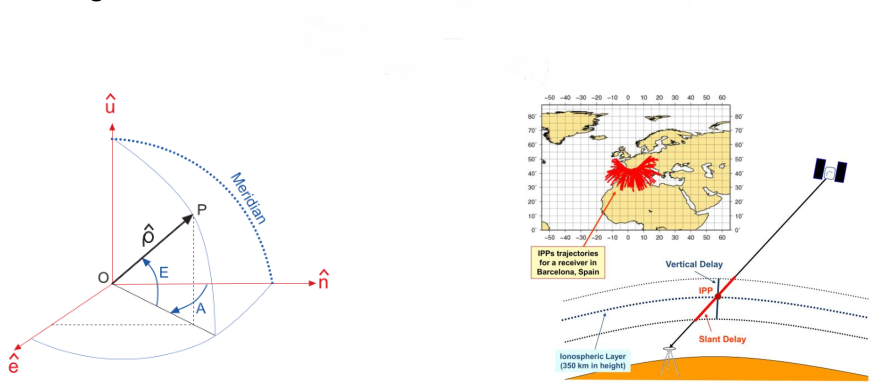
\includegraphics[width=0.9\textwidth]{elev}
	\caption{Kut elevacije (izvor)}
	\label{fig:elev}
\end{figure}

Ponovno lineariziramo desne strane jednadžbi \ref{eq:1partial} i dobivamo da $\forall i \in \{1,2,3,4, ...\}$
\begin{align*}
d_i - \sqrt{(x_k-x_i)^{2}+(y_k-y_i)^{2}+(z_k-z_i)^{2}} - c\cdot (d_T)_k & = \\
\frac{\partial f}{\partial x}\Delta x_k + \frac{\partial f}{\partial y}\Delta y_k + \frac{\partial f}{\partial z}\Delta z_k + \frac{\partial f}{\partial d_T}\Delta (d_T)_k &= 
\begin{bmatrix}
\frac{\partial f_i}{\partial x} &
\frac{\partial f_i}{\partial y} &
\frac{\partial f_i}{\partial z} &
\frac{\partial f_i}{\partial d_T}
\end{bmatrix}
\begin{bmatrix}
\Delta x \\
\Delta y \\
\Delta z \\
\Delta d_T
\end{bmatrix} \\ 
\end{align*}
gdje je $i$ indeks pridružen vrijednostima i-te jednadžbe sustava.

Općenito, $i$ može biti proizvoljan. 
Glavno da sadrži najmanje onoliko nezavisnih jednadžbi koliko sustav ima nepoznanica.
Do sada se većinom promatrao sustav $i = 4 = \textit{broj nepoznanica sustava}$ s međusobno nezavisnim jednadžbama. Nastavimo u istom tonu.
\\
Uz 
\begin{align}
\mathbf{A} & := \begin{bmatrix}
\frac{\partial f_1}{\partial x} &
\frac{\partial f_1}{\partial y} &
\frac{\partial f_1}{\partial z} &
\frac{\partial f_1}{\partial d_T} \\
\frac{\partial f_2}{\partial x} &
\frac{\partial f_2}{\partial y} &
\frac{\partial f_2}{\partial z} &
\frac{\partial f_2}{\partial d_T} \\
\frac{\partial f_3}{\partial x} &
\frac{\partial f_3}{\partial y} &
\frac{\partial f_3}{\partial z} &
\frac{\partial f_3}{\partial d_T} \\
\frac{\partial f_4}{\partial x} &
\frac{\partial f_4}{\partial y} &
\frac{\partial f_4}{\partial z} &
\frac{\partial f_4}{\partial d_T}
\end{bmatrix} \\
& = \begin{bmatrix}
\frac{(x-x_1)}{\sqrt{(x-x_1)^{2}+(y-y_1)^{2}+(z-z_1)^{2}}} & \frac{(y-y_1)}{\sqrt{(x-x_1)^{2}+(y-y_1)^{2}+(z-z_1)^{2}}} & \frac{(z-z_1)}{\sqrt{(x-x_1)^{2}+(y-y_1)^{2}+(z-z_1)^{2}}} & c \\
\frac{(x-x_2)}{\sqrt{(x-x_2)^{2}+(y-y_2)^{2}+(z-z_2)^{2}}} & \frac{(y-y_2)}{\sqrt{(x-x_2)^{2}+(y-y_2)^{2}+(z-z_2)^{2}}} & \frac{(z-z_2)}{\sqrt{(x-x_2)^{2}+(y-y_2)^{2}+(z-z_2)^{2}}} & c \\
\frac{(x-x_3)}{\sqrt{(x-x_3)^{2}+(y-y_3)^{2}+(z-z_3)^{2}}} & \frac{(y-y_3)}{\sqrt{(x-x_3)^{2}+(y-y_3)^{2}+(z-z_3)^{2}}} & \frac{(z-z_3)}{\sqrt{(x-x_3)^{2}+(y-y_3)^{2}+(z-z_3)^{2}}} & c \\
\frac{(x-x_4)}{\sqrt{(x-x_4)^{2}+(y-y_4)^{2}+(z-z_4)^{2}}} & \frac{(y-y_4)}{\sqrt{(x-x_4)^{2}+(y-y_4)^{2}+(z-z_4)^{2}}} & \frac{(z-z_4)}{\sqrt{(x-x_4)^{2}+(y-y_4)^{2}+(z-z_4)^{2}}} & c \\
\end{bmatrix}\\
\mathbf{x} & :=  \begin{bmatrix}
\Delta x \\
\Delta y \\
\Delta z \\
\Delta d_T
\end{bmatrix}\\
\mathbf{b} & := \begin{bmatrix}
d_1 - \sqrt{(x_k-x_1)^{2}+(y_k-y_1)^{2}+(z_k-z_1)^{2}} - c\cdot (d_T)_k \\
d_2 - \sqrt{(x_k-x_2)^{2}+(y_k-y_2)^{2}+(z_k-z_2)^{2}} - c\cdot (d_T)_k \\
d_3 - \sqrt{(x_k-x_3)^{2}+(y_k-y_3)^{2}+(z_k-z_3)^{2}} - c\cdot (d_T)_k \\
d_4 - \sqrt{(x_k-x_4)^{2}+(y_k-y_4)^{2}+(z_k-z_4)^{2}} - c\cdot (d_T)_k
\end{bmatrix}
\end{align}
imamo sustav:
\begin{align*}
\mathbf{A}\mathbf{x} = \mathbf{b}
\end{align*} i
\begin{align*}
\mathbf{p}(\mathbf{x}) := \mathbf{A}\mathbf{x} - \mathbf{b}
\end{align*}


Praksa nerjetko koristi samo jedan signal prilikom postupka procjene položaja i utjecaj ionosfere modelira 
na opisan način.

\subsubsection{Izvedba}
Prilikom izvedbe algoritma koristimo sustav s $i = 7$ jednadžbi.
Slijedi programski isječak koji izvodi opisanu metodu.
\begin{lstlisting}[language=R]
f
\end{lstlisting}
%TU stala 




\subsection{Usporedba osnovnog i poboljšanog algoritma} + zaključak zašto je bolji.

\section{Zaključak}
Potrebno promatrati i druge parametre, utjecaje refleksije, ionosfere itd.
%NAPIŠI I BEZ ONIH KVADRIRANJA I SRANJA == kako rademo u baski + vidi zasto te tezine
%; TOJE POČETNI ALG KOJI SMO MODIFICIRALI


%\label{stranica}
%Na stranici \pageref{stranica} se nalaza slika u \textbf{png} formatu.

\bibliographystyle{babamspl} % babamspl ili babplain

% U datoteku diplomski.bib se stavljaju bibliografske reference
% Bibliografske reference u bib formatu se mogu dobiti iz MathSciNet baze, Google Scholara, ArXiva, ...
\bibliography{diplomski}

\pagestyle{empty} % ne zelimo brojanje sljedecih stranica

% I na koncu idu sazeci na hrvatskom i engleskom

\begin{sazetak}
Satelitsko određivanje položja predstavlja temeljnu
tehnologiju rastućeg broja tehnoloških i društveno-ekonomskih sustava.
Kvaliteta njihovih
usluga određena je točnoću procjene položja
satelitskim sustavima.
Programski određen radioprijamnik za satelitsku navigaciju
procesira signale za određivanje položja i podatke
iz navigacijske poruke
u tri osnovne domene: radiofrekvencijskoj, u domeni osnovnog frekvencijskog
područja te u domeni navigacijske primjene.
Ovaj rad analizira postupak procjene položaja
u domeni navigacijske primjene. U tu svrhu, koriste se na osobnom računalu
izveden programski određen GPS prijamnik i ulazni podatci
o opaženim pseudoudaljenostima spremljeni
u RINEX podatkovnom formatu.
Analiza korištenog algoritma procjene položaja
temelji se na izmjerenim pseudoudaljenosti (Sanz Subirana et al, 2013, Chapter 6.1)
te se otkrivaju potencijalne slabosti algoritma
s učincima na točnost procjene položja. Na kraju, predlažu se poboljšanja
algoritma te ih se izvodi u programskom okruženju R. 
Poboljšanja algoritma su vrednovana komparativnom analizom obilježja
poboljšanog i izvornog algoritma.
\end{sazetak}

\begin{summary}
In this ...
\end{summary}

% te zivotopis

\begin{cv}
Dana ...
\end{cv}

\appendix

\chapter{Taylorov red potencija}\label{appendix:aTay}
Primjetimo kako smo na stranici \pageref{stranica:NGLin} pretpostavili
kako će za rezidualnu funkciju $\mathbf{p}(\mathbf{x})$ postojati njezin 
razvoj u Taylorov red oko svake točke $\mathbf{x_k}$. Ipak,
Taylorov red nije definiran za svaku funkciju na $\R^n, n \in \N$.
Prilikom primjene Iterativne metode najmanjih kvadrata, treba zahtjevati da 
funkcija $\mathbf{p}(\mathbf{x})$ i točka $x_k$ zadovoljava uvjete definicije razvoja funkcije u Taylorov red oko točke $x_k$ \cite{math:tay}.
\begin{defn}
	Naka je $f: \mathbf{I} \to \R $ funkcija klase $C^\infty(\mathbf{I})$ definirana
	na otvorenom intervalu $\mathbf{I} \subseteq \R^n$ i neka je $c \in \mathbf{I}$.
	Red potencija
	\begin{align}
	T \left[f,c\right] := \sum_{n=0}^{\infty} \frac{f^{(n)}}{n!} \left(x - c\right)^n
	\end{align}
	nazivamo \textbf{Taylorov red} funkcije $f$ oko točke $c$.
\end{defn}%

Također,
pretpostavlja se kako je 
\begin{align}\label{eg:a1}
	\mathbf{p}(\mathbf{x_{k+1}}+\Delta \mathbf{x}_k) = T \left[\mathbf{p},x_k \right]
\end{align}
što općenito nije točno.
Naime, Taylorov red $T \left[f,c\right] $ funkcije 
$f \in C^\infty(\mathbf{I})$ nužno ne konvergira za svaki $x \not = c, x \in \mathbf{I}$
ili može konvergirati prema nekoj drugoj funkciji.
Uvjete pod kojima zaista vrijedi \ref{eg:a1} opisani su teoremima u nastavku.

\begin{defn}[Analitička funkcija]
	Za $f \in C^\infty(\mathbf{I})$ kažemo da je \textbf{analitička u točki} $c \in \mathbf{I}$ ako njezin Taylorov red:
	\begin{align*}
		T \left[f,c\right] := \sum_{n=0}^{\infty} \frac{f^{(n)}}{n!} \left(x - c\right)^n
	\end{align*}
	
	ima radijus konvergencije $R > 0$ i ako postoji $0 < \delta \leq R$ takav da vrijedi 
	\begin{align*}
	f(x) = T \left[f,c\right] := \sum_{n=0}^{\infty} \frac{f^{(n)}}{n!} \left(x - c\right)^n,
	\forall x \in \left < c-\delta, c+\delta \right > \cap \mathbf{I}
	\end{align*}
	U oznaci: $f \in C^\omega(\mathbf{I})$.
\end{defn}
\begin{thm}\label{thm:konv1}
	Neka je $\sum_{n=0}^{\infty} a_n \left(x - c\right)^n$ red potencija s radijusom konvergencije $R > 0$. Za $\mathbf{I} := \left < c-R, c+R\right >$,
	funkcija $f: \mathbf{I} \to \R$ definirana s 
	\begin{align}
		f(x) := \sum_{n=0}^{\infty} a_n \left(x - c\right)^n
	\end{align}
	je analitička na čitavom $\mathbf{I}$. Nadalje, za svaki $\alpha \in \mathbf{I}$ 
	pripadni Taylorov red
	\begin{align}
		T \left[f,\alpha \right] = \sum_{n=0}^{\infty} \frac{f^{(n)}}{n!} \left(x - \alpha \right)^n
	\end{align}
	ima radijus konvergencije $\rho \leq R - (c - \alpha)$ i vrijedi 
	\begin{align}
	f(x) = T \left[f,\alpha \right] = \sum_{n=0}^{\infty} \frac{f^{(n)}}{n!} \left(x - \alpha \right)^n
	\end{align}
\end{thm}


\begin{thm}\label{thm:konv}
	Naka je $f: \mathbf{I} \to \R $ funkcija klase $C^\infty(\mathbf{I})$ definirana
	na otvorenom intervalu $\mathbf{I} \subseteq \R^n$.
	Tada je $f \in C^\omega(\mathbf{I}$ ako i samo ako za svaki $c \in \mathbf{I}$ postoje
	$\delta > 0$ i konstante $C > 0$ i $ r > 0 $ takve da za sve $n \in \Z_+$ vrijedi:
	\begin{align}
		\left | f^{n}(x)  \leq  C \frac{n!}{r^n}  \right | 
		\forall x \in \mathbf{J} := \left < c-\delta, c+\delta \right > \cap \mathbf{I}
	\end{align}
U tom slučaju $f(x) = T \left[f,c\right](x) $ $
\forall x \in \left < c-r, c+r \right > \cap \mathbf{J}$.
\end{thm}
Za primjenu iterativne metode
najmanjih kvadrata $\mathbf{p}$ mora biti klase $C^\infty(\mathbf{I})$ gdje je $\mathbf{I}$ unija otvorenih okolina oko svih izračinatih $\mathbf{x}_k, k \in \N$, osim zadnjega.
Također, otvorena okolina oko $\mathbf{x}_k$  mora barem sadržavaki otvorenu kuglu $K(\mathbf{x}_k,\Delta \mathbf{x}_k)$ i za $\mathbf{p}$ mora vrijediti teorem \ref{thm:konv1} ili  \ref{thm:konv}.

\chapter{Jakobijeva matrica funkcije $\mathbf{h}$, $J$}
Iz jednakosti \ref{eq:matrix2} i $J = \mathbf{p}(\mathbf{x})$ dobivamo
\begin{align}
J = \frac{\partial \mathbf{h}}{\partial \mathbf{x}}
\end{align}
Za 
\begin{align}
\mathbf{h} (\mathbf{x}) := 
\begin{bmatrix}
||(\mathbf{s}_1-\mathbf{x}_{1:3})|| \\
||(\mathbf{s}_2-\mathbf{x}_{1:3})|| \\
||(\mathbf{s}_3-\mathbf{x}_{1:3})||\\
\end{bmatrix} 
\end{align}
dobivamo
\begin{align}
J = \begin{bmatrix}
\frac{\partial}{\partial \mathbf{x}} ||(s_1-\mathbf{x}_{1:3})|| \\
\frac{\partial}{\partial \mathbf{x}} ||(s_2-\mathbf{x}_{1:3})||\\
\frac{\partial}{\partial \mathbf{x}} ||(s_3-\mathbf{x}_{1:3})|| 
\end{bmatrix}%
= - \begin{bmatrix}
\frac{(s_1-\mathbf{x}_{1:4})^T}{||(s_1-\mathbf{x}_{1:3})||} \\
\frac{(s_2-\mathbf{x}_{1:4})^T}{||(s_1-\mathbf{x}_{1:3})||}\\
\frac{(s_3-\mathbf{x}_{1:4})^T}{||(s_1-\mathbf{x}_{1:3})||} 
\end{bmatrix} = (J_n(1:3,1:3))
\end{align}
uz $\hat{\mathbf{x}} = \mathbf{x}_n$
\chapter{Mjere kvalitete "zviježđda"}\label{appendix:DOP}

\end{document}